\documentclass[12pt]{article}
\usepackage[T1]{fontenc}
\usepackage[utf8]{inputenc}
\usepackage[margin=1in]{geometry}
\usepackage[spanish]{babel}\decimalpoint
\usepackage{setspace}\onehalfspacing
\usepackage{parskip} %Espacio entre parrafos.
\usepackage{graphicx} %Para usar \includegraphics[]{}
\usepackage{amssymb} %Para usar el si­mbolo del conj. de los Reales.%
\usepackage{amsmath} % Para usar columnas vectoriales.
\usepackage{booktabs} % Para agregar \toprule y \bottomrule a tablas
\usepackage{hyperref} %Siempre debe ser el ultimo paquete.


\setlength{\parindent}{0pt} %Texto justificado.
\setcounter{tocdepth}{2} %Que no incluya subsubsections en el índice.


%===================================================================%

\title{Apuntes 'Calculus 1A: Differentiation'}
\author{}
\date{}

\begin{document}

\maketitle
\tableofcontents

\newpage



\section{Aproximaciones.}


\subsection{Aproximación Lineal: Error de Medición.}

En la semana anterior comenzamos estudiando la aproximación lineal.
Principalmente, vimos que es un método para estimar el output de una función (conocida o no) haciendo uso de la aproximación de la línea tangente (i.e., la derivada) en un punto de ella (e.g., estimar $\sqrt{104}$ sabiendo que $\sqrt{100} = 10$).

La idea central es que es mucho más fácil \textbf{linearizar una función} para estimar el output de una función más compleja (e.g., una función con $x^{5}$). No obtendremos el valor exacto, pero sí uno aceptablemente cercano.

En esta ocasión usaremos la aproximación lineal para desarrollar herramientas que nos permitirán observar, por ejemplo, cómo un error de medición se propaga en un sistema o para entender la sensibilidad de un sistema a pequeñas perturbaciones.

\subsubsection{Diseño de un Canopy (\textit{Ziplines}).}

Cuando se diseña un canopy, uno de los aspectos que se debe considerar cuidadosamente es la \textbf{velocidad} con la cual un usuario/a va a viajar a través de ésta.

La \textbf{velocidad de viaje en el canopy} va a depender de variables como el peso de quien viaja en ella y de fenómenos asociados al clima. Estas últimas no las podemos controlar, pero como tenemos un espacio horizontal fijo entre los dos árboles en los que se sostiene el cable del canopy, sí podemos mantener constante (i.e., podemos controlar) la \textbf{altura vertical total} recorrida a lo largo de éste.

\begin{figure}[hbt!]
\centering
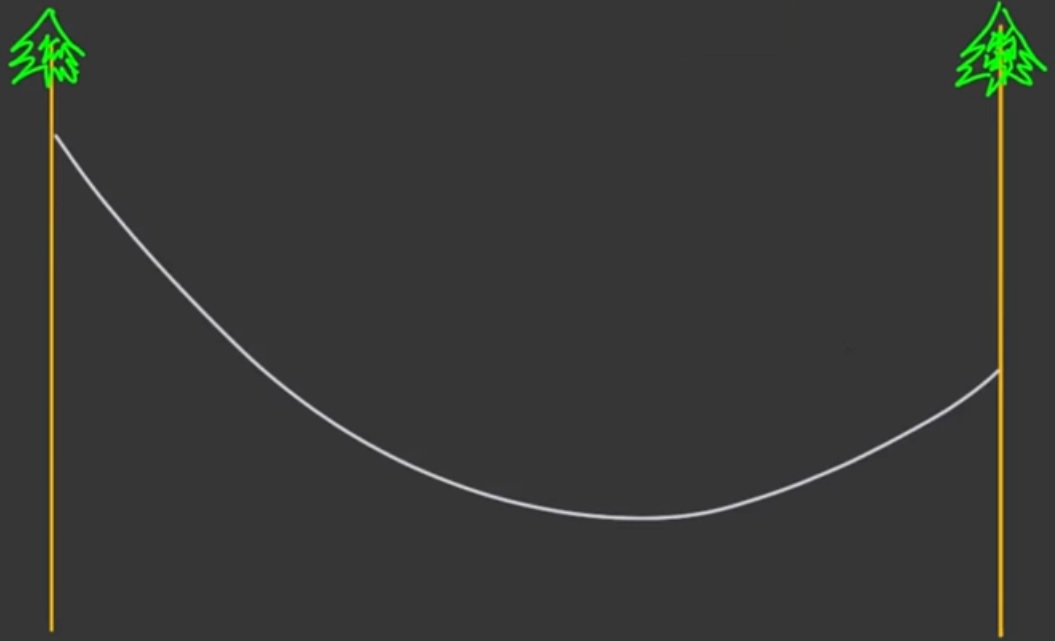
\includegraphics[scale=0.3]{img/zipline_example.jpg}
\end{figure}

En otras palabras, tenemos la opción de alterar la altura del canopy moviendo el cable más hacia arriba o hacia abajo. Si lo hacemos, dicho cambio tendrá un efecto en la velocidad del viaje.

Entonces, formalmente digamos que $h$ es la altura total del viaje en el canopy y $v$ es la velocidad máxima que se alcanzó en el trayecto. Nuestro objetivo es ver \textbf{a qué valor se aproxima la velocidad máxima que alcanza el canopy al modificar la altura del cable}:
\[\Delta v \approx \Delta h \text{ ??}\]

Un enfoque que podemos usar para resolver este problema, es la \textbf{ley de conservación de energía}.

Propuesta y probada en primera instancia por Émilie du Châtelet, la \href{https://en.wikipedia.org/wiki/Conservation_of_energy}{ley de conservación de la energía} señala que la energía no puede ser creada ni destruida, más bien solo puede ser transformada o transferida de una forma a otra (i.e., de un sistema a otro).

En otras palabras, esta ley establece que cuando una cantidad de una energía pasa a otro tipo de energía (i.e., de un sistema a otro), dicha cantidad seguirá siendo la misma. Es decir, \textbf{será constante}.

Por lo tanto, si denotamos a la energía total del sistema como $E$, entonces:
\[E_{\text{inicial}} = E_{\text{final}}\]
Por otra parte, acá nos concentraremos en un sistema ideal, donde no consideraremos la energía térmica (generada por fricción) o de resistencia al viento.

Así, diremos que $E$ se constituye como la suma de la energía de un objeto en descanso o Energía Potencial ($U$) y de la energía del mismo objeto en movimiento, también conocida como Energía Cinética ($K$).
\[U_{\text{inicial}} + K_{\text{inicial}} = U_{\text{final}} + K_{\text{final}}\]
Y como es energía ``conservada'', entonces cualquier cambio en una de las energías debe ir acompañado de un mismo cambio en la cantidad de la otra energía, pero en sentido opuesto.
\[\Delta U + \Delta K = 0\]
Tanto la energía potencial como la cinética tienen sus propias fórmulas:

\begin{itemize}
\item $U = mgh$
\item $K = \frac{1}{2}mv^{2}$
\end{itemize}

En el sistema del canopy, $m$ corresponde a la masa del viajero/a, $g$ es la fuerza gravitacional (constante), $h$ es la altura total que se alcanzó en el trayecto y, finalmente, $v$ es la velocidad máxima que se logró alcanzar.

En este caso estamos concentrados en la \textbf{velocidad máxima} que puede alcanzar el canopy, es decir, cuando deja de estar completamente en descanso, lo cual significa que $U = 0$ y, en consecuencia, el sistema total de energía será igual a $K$:
\[E_{\text{final}} = K = \frac{1}{2}mv^{2}\]
Podemos hacer uso de esta fórmula para conocer ver la velocidad máxima del canopy:
\[E = \frac{1}{2} \ mv^{2}\]
\[v^{2} = \frac{2E}{m}\]
\[v = \left(\frac{2E}{m}\right)^{1/2}\]
Esta fórmula corresponde a la \textbf{velocidad máxima en la altura original} (i.e, en $h$) del canopy. En otras palabras, aún no consideramos el cambio en ella y cómo afecta en la velocidad. 

Ahora bien, digamos que modificamos la altura $h$ en una pequeña cantidad $\Delta h$, tal como se ve en la siguiente figura.

\begin{figure}[hbt!]
\centering
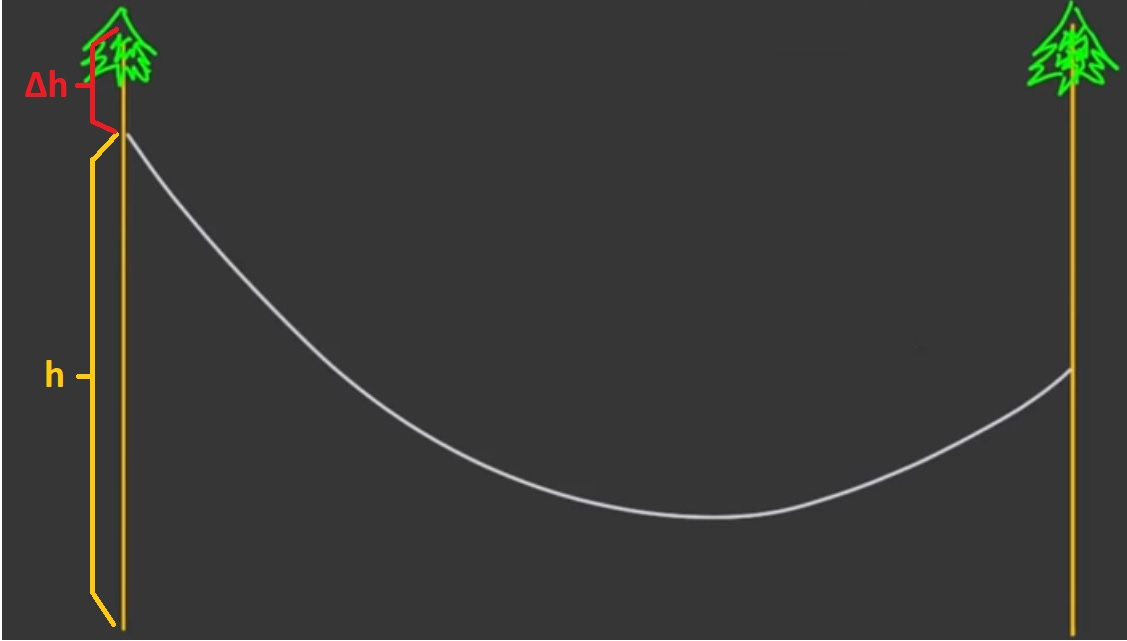
\includegraphics[scale=0.3]{img/zipline_example_2.jpg}
\end{figure}

A partir del enfoque de la ley de conservación de la energía, este pequeño cambio en la altura va a \textbf{alterar la energía total del sistema} porque vamos a estar \textbf{agregando o restando una pequeña cantidad de energía potencial}. En consecuencia, tendremos una nueva energía total del sistema:
\[E_{\text{final}} = K + mg\Delta h\]
Y sabemos que, en la energía total original, $E = K$. Por lo tanto:
\[E_{\text{final}} = E + mg\Delta h\]
Ahora necesitamos transformar toda esta pequeña energía potencial en energía cinética, ya que nos interesa ver cómo cambia la velocidad máxima. Esto significa que vamos a tener una nueva velocidad, a la cual denotaremos como $v_{f}$. En ese sentido, el cambio en la velocidad máxima $\Delta v$ será diferencia entre $v_{f}$ y la misma, pero en la altura original $h$, que corresponde a $v$.
\[\Delta v = v_{f} - v\]
A partir de la ecuación anterior, podemos obtener la nueva velocidad máxima:
\[v_{f} = v + \Delta v\]
Con esta información podemos calcular el cambio de la velocidad máxima que alcanza el canopy. Para ello, podemos usar la fórmula de la velocidad máxima, $v = \left(\frac{2E}{m}\right)^{1/2}$, pero para la nueva velocidad, que proviene del cambio en la altura o en la energía potencial:
\[v + \Delta v = \left(\frac{2(E + mg\Delta h)}{m}\right)^{1/2}\]
Despejemos $\Delta v$ y resolvamos un poco el lado derecho de la ecuación:
\[\Delta v = \left(\frac{2E}{m} + \frac{2mg\Delta h}{m}\right)^{1/2} - v\]
\[\Delta v = \left(\frac{2E}{m} + 2g\Delta h\right)^{1/2} - \left(\frac{2E}{m}\right)^{1/2}\]
\[\Delta v = \left(\frac{2E}{m}\right)^{1/2} \cdot \left(1 + \frac{mg \Delta h}{E}\right)^{1/2} - \left(\frac{2E}{m}\right)^{1/2}\]
\[\Delta v = \left(\frac{2E}{m}\right)^{1/2} \cdot \left[\left(1 + \frac{mg \Delta h}{E}\right)^{1/2} - 1 \right]\]
En este punto, usar esta ecuación para obtener el cambio en la velocidad máxima puede llegar a ser complicado, en particular por la expresión $\left(1 + \frac{mg \Delta h}{E}\right)^{1/2}$. Sin embargo, podemos reducir esta expresión por medio de una \textbf{linearización}. Es decir, calculamos la \textbf{aproximación lineal} en un punto para obtener de forma más fácil un valor \textbf{aproximado} de $\Delta v$.

Para hacerlo más sencillo y rápido, en vez de linearizar de inmediato  a $\left(1 + \frac{mg \Delta h}{E}\right)^{1/2}$, lo haremos con una función de la forma $(1 + u)^{r}$, donde $r$ es constante y $u$ variable.

En particular, veamos a qué valor se aproxima\footnote{Fórmula de la aproximación lineal: \[f(x) \approx f(x_{0}) + \left.\frac{d}{dx} f(x) \right|_{x = x_{0}} \cdot (x - x_{0})\]} $(1 + u)^{r}$ cuando nos acercamos al punto $u = 0$.
\[(1 + u)^{r} \approx (1 + 0)^{r} + \left.\frac{d}{du} (1 + u)^{r} \right|_{u = 0} \cdot (u - 0)\]
\[(1 + u)^{r} \approx 1 + \left.\frac{d}{du} (1 + u)^{r} \right|_{u = 0} \cdot u\]
Calculemos de forma separada la derivada del lado derecho de la aproximación.
\[\frac{d}{du} (1 + u)^{r} = \frac{d}{d(1 + u)} (1 + u)^{r} \cdot \frac{d}{du} (1 + u) = r \ (1 + u)^{r - 1}\]
Luego, obtengamos la derivada de $(1 + u)^{r}$ en $u = 0$.
\[\left.\frac{d}{du} (1 + u)^{r} \right|_{u = 0} = r \ (1 + 0)^{r - 1} = r\]
Veamos finalmente cuál es la aproximación lineal de $(1 + u)^{r}$ en $u = 0$:
\[(1 + u)^{r} \approx 1 + ru\]
Entonces usaremos esta forma de la aproximación lineal para linearizar a $\left(1 + \frac{mg \Delta h}{E}\right)^{1/2}$. Si nos basamos en la función que acabamos de aproximar, entonces lo que haremos es ver a qué se aproxima $\left(1 + \frac{mg \Delta h}{E}\right)^{1/2}$ cuando nos acercamos a $\frac{mg \Delta h}{E} = 0$.

Por lo tanto, si $r = \frac{1}{2}$ y $u = \frac{mg \Delta h}{E}$, entonces:
\[\left(1 + \frac{mg \Delta h}{E}\right)^{1/2} \approx 1 + \frac{1}{2} \cdot \frac{mg \Delta h}{E} = 1 + \frac{mg \Delta h}{2E}\]

\newpage

La expresión $\frac{mg \Delta h}{2E}$ también podemos denotarla como $\frac{m}{2E} \cdot g \Delta h$. Si observamos bien, podemos decir que $\frac{m}{2E} = v^{-2}$, lo que nos permite para simplificar la expresión que obtuvimos en la aproximación.
\[\left(1 + \frac{mg \Delta h}{E}\right)^{1/2} \approx 1 + \frac{g \Delta h}{v^{2}}\]
Entonces agregaremos esta linearización a la fórmula para obtener el cambio en la velocidad máxima del canopy $\Delta v$, pero ahora su valor será aproximado:
\[\Delta v \approx \left(\frac{2E}{m}\right)^{1/2} \cdot \left[1 + \frac{g \Delta h}{v^{2}} - 1 \right]\]
Por otra parte, $v = \left(\frac{2E}{m}\right)^{1/2}$, implicando que:
\[\Delta v \approx v \cdot \frac{g \Delta h}{v^{2}} = \frac{g \Delta h}{v}\]
Entonces, ayudándonos de la aproximación lineal de una expresión logramos obtener una fórmula más sencilla para ver cómo pequeños cambios en la altura del canopy afectarán a la velocidad máxima que se puede alcanzar en ella.

Veamos un ejemplo.

\underline{Ejemplo}: Digamos que la velocidad máxima que alcanza una persona en un viaje en canopy, es de $12 \ m/s$ y queremos saber a qué velocidad puede acercarse si cambiamos la altura del canopy en $0.1 \ m$ (i.e., en $10 \ cm$). Asumamos que la fuerza de gravedad $g = 10 \ m/s^{2}$.

\underline{Respuesta}: Reemplacemos dichos valores en la fórmula que acabamos de obtener:
\[\Delta v \approx \frac{g \Delta h}{v} =  \frac{10 \ m/s^{2} \cdot 0.1 \ m}{12 \ m/s} = 0.08 \ m/s\]
Por lo tanto, si aumentamos en $0.1 \ m$ la altura del canopy, el cambio en la velocidad máxima será, aproximadamente, de $0.08 \ m/s$. Si bien es poco este aumento, es posible que sea lo suficiente como para que el trayecto pueda realizarse completamente.

Revisemos otro caso.

\underline{Ejemplo}: Simplifiquemos otro supuesto. Digamos que una persona comienza su viaje a través del canopy sin impulsarse (i.e., en descanso). Esto implica que, al comienzo, la energía kinética es igual a cero. Por lo tanto, la energía total $E = U + K$ será:
\[E = mgh + 0 = mgh\]
Con este nuevo supuesto, digamos que cambiamos la altura de desplazo durante el viaje en un 2\%, es decir, $\frac{\Delta h}{h} = 0.02$. ¿En qué porcentaje cambió $v$?

\underline{Respuesta}: En este caso nos consultan sobre la proporción del cambio de la velocidad máxima al modificar la altura en un 2\%. Es decir, sobre $\frac{\Delta v}{v}$.

En ese sentido, la velocidad máxima seguirá siendo\footnote{Recordemos que estamos en un sistema de energía conservada} $v = \left(\frac{2E}{m}\right)^{1/2}$, pero ahora estamos bajo el supuesto en que la persona en el canopy parte en descanso, lo que implica que $E = mgh$. Por lo tanto, la velocidad se calculará de la siguiente manera:
\[v = \left(\frac{2mgh}{m}\right)^{1/2} = (2gh)^{1/2}\]
Y como modificamos la altura, tendremos que calcular una nueva velocidad ($v_{f} = \Delta v + v$) considerando una nueva altura ($h_{f} = \Delta h + h$). En consecuencia:
\[\Delta v + v = \left[2g(h + \Delta h)\right]^{1/2}\]
Resolvamos la ecuación para $\Delta v$:
\[\Delta v = \left[2g(h + \Delta h)\right]^{1/2} - v\]
También, sabemos que $v = (2gh)^{1/2}$ y podemos factorizar la expresión que hay en el paréntesis cuadrado:
\[\Delta v = \left[2gh \cdot \left(1 + \frac{\Delta h}{h}\right)\right]^{1/2} - (2gh)^{1/2}\]
Lo anterior es lo mismo que:
\[\Delta v = \left(2gh\right)^{1/2} \cdot \left(1 + \frac{\Delta h}{h}\right)^{1/2} - (2gh)^{1/2} = \left(2gh\right)^{1/2} \cdot \left[\left(1 + \frac{\Delta h}{h}\right)^{1/2} - 1\right]\]
Finalmente, como $v =(2gh)^{1/2}$, entonces:
\[\Delta v = v \cdot \left[\left(1 + \frac{\Delta h}{h}\right)^{1/2} - 1\right]\]
\[\frac{\Delta v}{v} = \left(1 + \frac{\Delta h}{h}\right)^{1/2} - 1\]
Ahora bien, si nos damos cuenta, podemos linearizar esta fórmula tomando la aproximación lineal de $\left(1 + \frac{\Delta h}{h}\right)^{1/2}$ basados en $(1 + u)^{r} \approx 1 + ru$ cuando $u \to 0$. En este caso, lo haremos asumiendo que $\frac{\Delta h}{h} \to 0$. Por lo tanto:
\[\frac{\Delta v}{v} \approx 1 + \frac{1}{2} \cdot \frac{\Delta h}{h} - 1 = \frac{1}{2} \cdot \frac{\Delta h}{h}\]
En el ejemplo nos señalan que la altura del canopy fue modificada en un 2\%, lo que quiere decir que:
\[\frac{\Delta v}{v} \approx \frac{1}{2} \cdot \frac{2}{100} = 0.01\]
En otras palabras, al cambiar en un 2\% la altura del canopy, si una persona parte en reposo, entonces su velocidad máxima cambiará en un 1\%, aproximadamente.


\subsubsection{Combinando aproximaciones de sumas, productos y composiciones.}

Vayamos a la fórmula para calcular aproximaciones lineales y resolvámosla bajo el caso en que \textbf{nos acercamos a $x = 0$}.
\[f(x) \approx f(0) + \left. \frac{d}{dx} f(x) \right|_{x = 0} \cdot (x - 0)\]
\[f(x) \approx f(0) + \left. \frac{d}{dx} f(x) \right|_{x = 0} \cdot x\]
Esta fórmula la podemos usar para linearizar funciones básicas \textbf{cuando nos acercamos a $x = 0$}. Por ejemplo, veamos los casos de las funciones $\sin(x)$, $\cos(x)$, $e^{x}$ y $\ln(1 + x)$.
\[\sin(x) \approx \sin(0) + \left. \frac{d}{dx} \sin(x) \right|_{x = 0} \cdot x \approx x\]
\[\cos(x) \approx \cos(0) + \left. \frac{d}{dx} \cos(x) \right|_{x = 0} \cdot x \approx 1\]
\[e^{x} \approx e^{0} + \left. \frac{d}{dx} e^{x} \right|_{x = 0} \cdot x \approx 1 + x\]
\[\ln(1 + x) \approx \ln(1 + 0) + \left. \frac{d}{dx} \ln(1 + x) \right|_{x = 0} \cdot x \approx x\]

\newpage

Por lo tanto, cuando nos acercamos al punto $x = 0$, entonces:

\begin{itemize}
\item $(1 + u)^{r} \approx 1 + ru$
\item $\sin(x) \approx x$
\item $\cos(x) \approx 1$
\item $e^{x} \approx 1 + x$
\item $\ln(1 + x) \approx x$
\end{itemize}

Estas funciones, que son básicas y sabemos cómo derivarlas, nos pueden servir para aproximar linealmente funciones más complejas cuando $x \to 0$.

\underline{Ejemplo}: Busque la aproximación lineal cercano a $x = 0$ de: 1) $\sin(x) + \ln(1 + x)$ y 2) $3e^{x}$.

\underline{Respuesta}: Usemos las fórmulas que acabamos de obtener para linearizar estas funciones.

\begin{enumerate}
\item $\sin(x) + \ln(1 + x) \approx x + x = 2x$
\item $3e^{x} \approx 3 \cdot (1 + x) \approx 3 + 3x$
\end{enumerate}

También podemos obtener la aproximación lineal de \textbf{funciones compuestas} cuando $x \to 0$.

Por ejemplo, en el caso del canopy trabajamos con una función de la forma $(1 + ax)^{1/2}$ y asignamos el producto $ax$ a una variable $u$ (i.e., $ax = u$), llevándonos a establecer que:
\[(1 + ax)^{1/2} = (1 + u)^{1/2}\]
Entonces, si $x \to 0$, en consecuencia $ax \to 0$ y $u \to 0$, lo que implica que:
\[(1 + ax)^{1/2} = (1 + u)^{1/2} \approx 1 + \frac{1}{2} \cdot u = 1 + \frac{ax}{2}\]
En este ejemplo, la función compuesta fue solo un factor escalar lineal ($ax$), pero este enfoque funciona en general.

\underline{Ejemplo}: Busque una aproximación lineal para $\ln(u)$ cerca del punto $u = 1$.

\underline{Respuesta}: Sabemos que $\ln(1 + x) \approx x$ cuando $x\to 0$, entonces podemos establecer que $u = 1 + x$. Por lo tanto:
\[\ln(u) = \ln(1 + x)\]
Lo anterior hace sentido ya que, cuando $x \to 0$, entonces $u \to 1$. De este modo, usaremos la aproximación lineal $\ln(1 + x)$ cuando $x \to 0$ en la igualdad de arriba.
\[\ln(u) = \ln(1 + x) \approx x\]
Finalmente, resolvemos la ecuación $u = 1 + x$ para $x$, que resulta en $x = u - 1$ y la reemplazamos en la aproximación que acabamos de obtener.
\[\ln(u) \approx u - 1\]
\underline{Ejemplo}: Busque la aproximación lineal cercana al punto $x = 0$ de $(4 + \sin(x))^{3/2}$.

\underline{Respuesta}: La función se parece a $(1 + x)^{r}$. Para acercarnos a ella, factoricémosla por $4^{3/2}$.
\[(4 + \sin(x))^{3/2} = 4^{3/2} \cdot \left(1 + \frac{\sin(x)}{4}\right)^{3/2}\]
Luego, establezcamos que $u = \frac{\sin(x)}{4}$.
\[4^{3/2} \cdot (1 + u)^{3/2} = 8 \cdot (1 + u)^{3/2}\]
Y sabemos que cuando $x \to 0$, entonces $(1 + x)^{r} \approx 1 + rx$.
\[8 \cdot (1 + u)^{3/2} \approx 8 \cdot \left(1 + \frac{3}{2} \cdot u\right)\]
Como $u = \frac{\sin(x)}{4}$, entonces:
\[8 \cdot (1 + u)^{3/2} \approx 8 \cdot \left(1 + \frac{3}{2} \cdot \frac{\sin(x)}{4}\right)\]
Esta función podemos seguir linearizándola, ya que sabemos que $\sin(x) \approx x$ cuando $x \to 0$.
\[8 \cdot \left(1 + \frac{3}{2} \cdot \frac{\sin(x)}{4}\right) \approx 8 \cdot \left(1 + \frac{3x}{8}\right)\]
En conclusión, cuando $x \to 0$, entonces $(4 + \sin(x))^{3/2} \approx 8 \cdot \left(1 + \frac{3x}{8}\right)$.

\subsubsection{Aproximaciones (probablemente no lineales) de funciones compuestas.}

Hasta ahora hemos visto ejemplos en donde comenzamos con una aproximación lineal y terminamos con una función lineal, pero éste no es siempre el caso.

\underline{Ejemplo}: Busque la aproximación lineal de $(1 + x^{2})^{-1}$ cercano al punto $x = 0$.

\underline{Respuesta}: Comencemos estableciendo que $u = x^{2}$, porque a medida que $x \to 0$, $u$ también lo hace.
\[(1 + x^{2})^{-1} = (1 + u)^{-1}\]
Entonces, mientras $u \to 0$, obtendremos que:
\[(1 + u)^{-1} \approx 1 - u\]
Y como $u = x^{2}$, por consiguiente:
\[(1 + x^{2})^{-1} \approx 1 - x^{2}\]
Como podemos observar, \textbf{realizamos una aproximación lineal}, pero terminamos con $1 - x^{2}$ que \textbf{no es una función lineal}. Esto se debe a que la linearización de $x^{2}$ cercano al punto $x = 0$, es $x^{2} \approx 0$.

Por otra parte, no olvidemos que $x^{2} \approx 0$ solo cuando $x \to 0$. En cualquier otro caso, no se aplica.

Veamos más formalmente la linearización de funciones compuestas que no siempre serán lineales.

Supongamos que $g(x)$ es una función tal que $g(0) = 0$. Para encontrar la aproximación de $f(g(x))$ cerca del punto $x = 0$, podemos establecer que $u = g(x)$. Por lo tanto:
\[f(u) \approx f(0) + \left. \frac{d}{du} f(u) \right|_{u = 0} \cdot u\]
Posteriormente, podemos reemplazar $u$ por $g(x)$, lo que nos lleva a:
\[f(g(x)) \approx f(g(0)) + \left. \frac{d}{dx} f(g(x)) \right|_{x = 0} \cdot g(x)\]
Esta fórmula para aproximar una función compuesta \textbf{solo se aplica para $g(0) = 0$}.

\newpage

\subsubsection{Aproximación Lineal del Producto de Funciones.}

Veamos el siguiente ejemplo.

\underline{Ejemplo}: Busque la aproximación lineal de la función $\frac{e^{-3x}}{\sqrt{1 + x}}$ cerca del punto $x = 0$.

\underline{Respuesta}: Podemos reescribir $\frac{e^{-3x}}{\sqrt{1 + x}}$ como:
\[e^{-3x} \cdot (1 + x)^{-1/2}\]
En este caso, la función es el producto de dos funciones compuestas, las que son idénticas a $e^{x}$ y $(1 + x)^{r}$, respectivamente, las cuales sabemos cómo linearizar cuando $x \to 0$ (pág. 10).
\[e^{-3x} \cdot (1 + x)^{-1/2} \approx (1 - 3x) \cdot \left(1 - \frac{x}{2}\right)\]
\[e^{-3x} \cdot (1 + x)^{-1/2} \approx 1 - \frac{7}{2}x + \frac{3}{2}x^{2}\]
Luego, eliminamos $\frac{3}{2}x^{2}$. En primer lugar, porque es un término insignificante. Por ejemplo, si $x = \frac{1}{100}$, entonces $x^{2} = \frac{1}{10000}$. Es decir, a medida que $x \to 0$, $x^2$ va a ser tan chico que no afectará en absoluto el valor al que nos aproximamos.

En segundo lugar, cancelaremos $\frac{3}{2}x^{2}$ puesto que no hace sentido. El término $x^{2}$ está haciendo referencia a que hay una curvatura cuadrática, sin embargo, en la función inicial no hay un término de ese orden. Haría sentido si estuviera desde un comienzo.

Por lo tanto, la aproximación lineal será:
\[e^{-3x} \cdot (1 + x)^{-1/2} \approx 1 - \frac{7}{2}x\]
En términos generales, para buscar la aproximación lineal de una función $h(x) = f(x)g(x)$ cerca de $x = 0$, \textbf{basta con encontrar las aproximaciones lineales por separado de $f(x)$ y $g(x)$} y luego se multiplican para encontrar la linearización final. Si aparecen términos cuadráticos o superiores, los eliminamos.

Entonces, sea $h(x) = f(x)g(x)$, busquemos su aproximación lineal mientras $x \to 0$ y partamos linealizando $f(x)$ y $g(x)$ cerca de $x = 0$. Por un tema de orden y espacio, usaré la notación de Newton para las derivadas.
\[f(x) \approx f(0) + f'(0) \cdot x \quad \text{y} \quad g(x) \approx g(0) + g'(0) \cdot x\]
Por lo tanto, la aproximación lineal de $h(x)$ cerca de $x = 0$ será el producto de las linealizaciones de $f(x)$ y $g(x)$:
\[h(x) \approx (f(0) + f'(0) \cdot x) \cdot (g(0) + g'(0) \cdot x)\]
\[h(x) \approx f(0)g(0) + f(0)g'(0)x + f'(0)g(0)x + f'(0)g'(0)x^{2}\]
Luego, eliminamos la expresión $f'(0)g'(0)x^{2}$, debido al término cuadrático:
\[h(x) \approx f(0)g(0) + f(0)g'(0)x + f'(0)g(0)x\]
Finalmente, factorizamos $f(0)g'(0)x + f'(0)g(0)x$ por $x$, que es su término común, obteniendo así una \textbf{fórmula para calcular la aproximación lineal del producto de dos funciones a medida que $x \to 0$}.
\[h(x) \approx f(0)g(0) + (f(0)g'(0) + f'(0)g(0)) \cdot x\]

\underline{Ejemplo}: Busque la aproximación lineal para $\ln(x)\sin(x - 1)$ cerca de $x = 1$.

\underline{Respuesta}: Para usar las aproximaciones lineales que ya conocemos para el logaritmo y para el seno, podemos establecer que $u = x - 1$. Primero, porque podemos usar $u$ en el seno; y, en segundo lugar, debido a que si despejamos $x$ en aquella igualdad, entonces $x = 1 + u$, la cual podemos usar en el logaritmo. Por lo tanto, a medida que $u \to 0$:
\[\ln(1 + u) \sin(u) \approx u \cdot u = u^{2} = 0\]
\underline{Ejemplo}: Busque la aproximación lineal para $\frac{\sin(x)}{\cos^{2}(x)}$ cerca de $x = 0$.

\underline{Respuesta}: Es posible reescribir $\frac{\sin(x)}{\cos^{2}(x)}$ como:
\[\sin(x) \cdot \cos^{-2}(x)\]
Finalmente, solo tenemos que linealizar ambos factores a medida que nos acercamos a $x = 0$. Solo no debemos olvidar que, luego de obtener la aproximación lineal de $\cos(x)$, tenemos que elevarla al cuadrado.
\[\sin(x) \cdot \cos^{-2}(x) \approx x \cdot (1)^{2} = x\]

\subsubsection{Error de Medición.}

Cuando realizamos algún tipo de medición, generalmente lo que obtenemos es una \textbf{estimación del valor exacto}, porque siempre hay factores externos que alterarán el resultado final. En ese sentido, siempre debemos considerar que habrá un \textbf{término de error} y lo podemos conocer con la ayuda de la aproximación lineal.

En cuanto al \textbf{término de error}, debemos entenderlo como la subestimación o sobreestimación del valor real que medimos. En otras palabras, lo interpretamos como un \textbf{intervalo cerrado en donde se ubica el valor real}.

\underline{Ejemplo}: Suponga que calculamos la velocidad de un objeto que viaja 1.2 metros en 1 segundo. El error de medición fue de 0.001 metros para la distancia y 0.01 segundos para el tiempo. ¿Cuál es el valor absoluto del error en la aproximación lineal para la velocidad?

\underline{Respuesta}:  Comencemos estableciendo que $x$ es la distancia en metros, mientras que $t$ es el tiempo en segundos. Por lo tanto, la velocidad $v$ la medimos como:
\[v = \frac{x}{t} \ m/s\]
Por otra parte, estamos asumiendo que la medida de la distancia y la del tiempo son distintas, cuya diferencia con las que obtuvimos son $\Delta x$ y $\Delta t$, respectivamente. En consecuencia, lo anterior también aplica para la velocidad, cuya diferencia será $\Delta v$. Por consiguiente, la velocidad real será la siguiente:
\[v + \Delta v = \frac{x + \Delta x}{t + \Delta t}\]
La fracción de la ecuación podemos escribirla también como $(x + \Delta x) \cdot (t + \Delta t)^{-1}$; y como estamos interesados en $\Delta v$, la despejamos, obteniendo que:
\[\Delta v = (x + \Delta x) \cdot (t + \Delta t)^{-1} - v\]
Factoricemos $(t + \Delta t)^{-1}$ por $t^{-1}$, que es igual a $\frac{1}{t}$. Por otra parte, recordemos que $v = \frac{x}{t}$.
\[\Delta v = \left[(x + \Delta x) \cdot \frac{1}{t} \cdot \left(1 + \frac{\Delta t}{t}\right)^{-1}\right] - \frac{x}{t}\]
Para tener una fórmula más sencilla de calcular, podemos linealizar el factor $\left(1 + \frac{\Delta t}{t}\right)^{-1}$ a medida que $\frac{\Delta t}{t} \to 0$.
\[\Delta v \approx \left[(x + \Delta x) \cdot \frac{1}{t} \cdot \left(1 - \frac{\Delta t}{t}\right)\right] - \frac{x}{t}\]
Aprovechemos que ahora el lado derecho es una expresión lineal, para simplificarla lo más posible.
\[\Delta v \approx \left[\left(\frac{x}{t} + \frac{\Delta x}{t}\right) \cdot \left(1 - \frac{\Delta t}{t}\right)\right] - \frac{x}{t}\]
\[\Delta v \approx - \frac{x \Delta t}{t^{2}} + \frac{\Delta x}{t} - \frac{\Delta x \Delta t}{t^{2}}\]
El termino $\frac{\Delta x \Delta t}{t^{2}}$ es cuadrático, así que lo eliminamos. Por lo tanto, el error de medición aproximado de la velocidad, se calcula como sigue:
\[\Delta v \approx \frac{\Delta x}{t} - \frac{x \Delta t}{t^{2}}\]
Recordemos que nos consultan sobre el valor absoluto del término de error de la velocidad. Es decir:
\[|\Delta v| \approx \left|\frac{\Delta x}{t} - \frac{x \Delta t}{t^{2}}\right|\]
Ante lo anterior, debemos aplicar algunas propiedades del valor absoluto. En primer lugar, $|a - b| \leq |a - c| + |b - c|$ (principio de subaditividad). Acá asumiremos que $c = 0$. Y, en segunda instancia, $\left| \frac{a}{b} \right| = \frac{|a|}{|b|}$. Lo que implica que:
\[|\Delta v| \leq \frac{|\Delta x|}{|t|} + \frac{|x \Delta t|}{|t^{2}|}\]
A partir de lo anterior, señalamos que los términos de error para la distancia y el tiempo serán $\Delta x \leq \pm 0.001 \ m$ y $\Delta \leq \pm 0.01 \ s$, respectivamente. Por lo tanto, el valor absoluto del término de error de la velocidad, es:
\[|\Delta v| \leq \frac{|\pm 0.001|}{|1|} \left(\frac{m}{s}\right) + \frac{|1.2 \cdot \pm 0.01|}{|1|} \left(\frac{m}{s}\right)\]
\[|\Delta v| \leq 0.013 \left(\frac{m}{s}\right)\]
\underline{Ejemplo}: Suponga que medimos la velocidad de un mosquito y obtuvimos que es igual a 1.3 m/s, con un error de 0.2 m/s. En cuanto a su peso, decidimos aproximarlo al de un grano de arroz, el cual es cercano a $10^{-6}$ kg. ¿Cuál es el error de la energía cinética? Asuma que no hay velocidad rotacional.

\underline{Respuesta}: Recordemos que la energía cinética se mide como:
\[K = \frac{1}{2} m v^{2}\]
En este ejemplo nos piden calcular $\Delta K$, ya que estamos considerando el término de error en la velocidad medida o $\Delta v$. Por consiguiente, la energía cinética real se calcula como:
\[K + \Delta K = \frac{1}{2} m (v + \Delta v)^{2}\]
Reemplacemos $K$ por $\frac{1}{2}mv^{2}$, despejemos $\Delta K$ y simplifiquemos lo más posible.
\[\Delta K = \frac{1}{2} mv^{2} \left(1 + \frac{\Delta v}{v}\right)^{2} - \frac{1}{2}mv^{2}\]
\[\Delta K = \frac{1}{2} mv^{2} \left[\left(1 + \frac{\Delta v}{v}\right)^{2} - 1\right]\]
Para facilitar el cálculo de $\Delta K$, podemos linearizar $\left(1 + \frac{\Delta v}{v}\right)^{2}$ a medida que $\frac{\Delta v}{v} \to 0$.
\[\Delta K \approx \frac{1}{2} mv^{2} \left[1 + \frac{2\Delta v}{v} - 1\right]\]
\[\Delta K \approx m v \Delta v\]
Finalmente, reemplazamos con los valores que nos dan en el ejemplo.
\[\Delta K \approx 10^{6} \cdot 1.3 \cdot 0.2 \left(kg \ m/s\right) = 2.6 \times 10^{-7} \ kg \ m^{2}/s^{2}\]
Podemos concluir que el término de error de la energía cinética fue, aproximadamente, de $2.6 \times 10^{-7} \ kg \ m^{2}/s^{2}$.

\newpage

\subsection{Aproximación Cuadrática.}

\subsubsection{La Línea de Mejor Ajuste.}

Realicemos un pequeño repaso sobre la definición de la derivada y la aproximación lineal.

Sea $f(x)$ una función continua. Su derivada en $\mathbb{R}$ se define como:
\[f'(x) = \lim_{\Delta x \to 0} \frac{f(x + \Delta x) - f(x)}{\Delta x}\]
Si restringimos la pendiente de la línea tangente de $f(x)$ en un punto $x = a$, entonces:
\[f'(a) = \lim_{\Delta x \to 0} \frac{f(a + \Delta x) - f(a)}{\Delta x}\]
Digamos que $x = a$ es el punto inicial de la línea secante de $f(x)$ que se acerca a ser la tangente mientras $\Delta x \to 0$. A partir de aquello se puede señalar que $\Delta x = x - a$ y, a su vez, que $x = \Delta x + a$. La última ecuación implica que si $\Delta x \to 0$, entonces $x \to a$. Por lo tanto:
\[f'(a) = \lim_{x \to a} \frac{f(x) - f(a)}{x - a}\]
La ecuación de arriba también podemos intepretarla como la aproximación de la pendiente de la línea secante a la pendiente de la línea tangente en $f(a)$.
\[\frac{f(x) - f(a)}{x - a} \approx f'(a)\]
Si despejamos $f(x)$, obtendremos la fórmula de la aproximación lineal en $x = a$ de dicha función.
\[f(x) \approx f(a) + f'(a)(x - a)\]
Todo esto ya lo hemos estudiado, pero algo que ignoramos es que el \textbf{lado derecho} de la aproximación lineal, es un polinomio de primer grado o, en otras palabras, una \textbf{ecuación lineal} de la forma $a + bx$, donde:

\begin{itemize}
\item $a \rightarrow f(a)$.
\item $bx \rightarrow f'(a)(x - a)$.
\end{itemize}

Que la fórmula de la aproximación lineal en un punto sea una ecuación lineal, no debería extrañarnos, ya que también porque proviene de la línea tangente de una función derivable, como lo acabamos de ver.

\newpage

Por otra parte, como en la aproximación lineal también estamos haciendo uso de la línea tangente a nivel geométrico, también podemos expresarla como una \textbf{función lineal}. En particular, la asignaremos a $L(x)$.
\[L(x) = f(a) + f'(a)(x - a)\]
Un aspecto interesante a destacar, es que si $L(x)$ toma el valor del punto de origen de la aproximación lineal (i.e, $x = a$), entonces será igual al output en el mismo punto de la función original.
\[L(a) = f(a) + f'(a)(a - a)\]
\[L(a) = f(a)\]
Otra característica no menor, es que $L(x)$ tiene su primera derivada, la que corresponde a una función constante\footnote{No olvidar que $f(a)$ y $f'(a)$, son constantes.} y que coincide con la derivada de la función original $f(x)$ en $x = a$, el punto de donde proviene la aproximación lineal.
\[L'(x) = 0 + f'(a)(1 - 0)\]
\[L'(x) = f'(a)\]
Por lo tanto, $L'(x)$ en $x = a$, será:
\[L'(a) = f'(a)\]
Entonces, debido a que $L(x)$ y $L'(x)$ en $x = a$ son iguales a $f(x)$ y $f'(x)$, respectivamente y en el mismo punto, se señala que la \textbf{aproximación lineal} es la \textbf{\underline{línea} de mejor ajuste de una función en el punto $x = a$}.


\subsubsection{La Parábola de Mejor Ajuste.}

Como dijimos anteriormente, la aproximación lineal de una función en un punto es la linea de mejor ajuste en esa ubicación. Y en valores muy cercanos, sigue siendo una buena estimación.

Por ejemplo, aproximemos el valor de $\cos\left(\frac{\pi}{8}\right)$ en $x \approx 0$.

Sabemos que en $x \approx 0$, $\cos(x) \approx 1$. En otras palabras:
\[L(x) = 1\]
Como $L(x)$ es una función constante, entonces en $L\left(\frac{\pi}{8}\right) = 1$.

\newpage

Usando calculadora, obtendremos que $\cos\left(\frac{\pi}{8}\right) \approx 0.92387$, un valor muy cercano a 1. Veamos gráficamente aquella proximidad de los resultados.

\begin{figure}[hbt!]
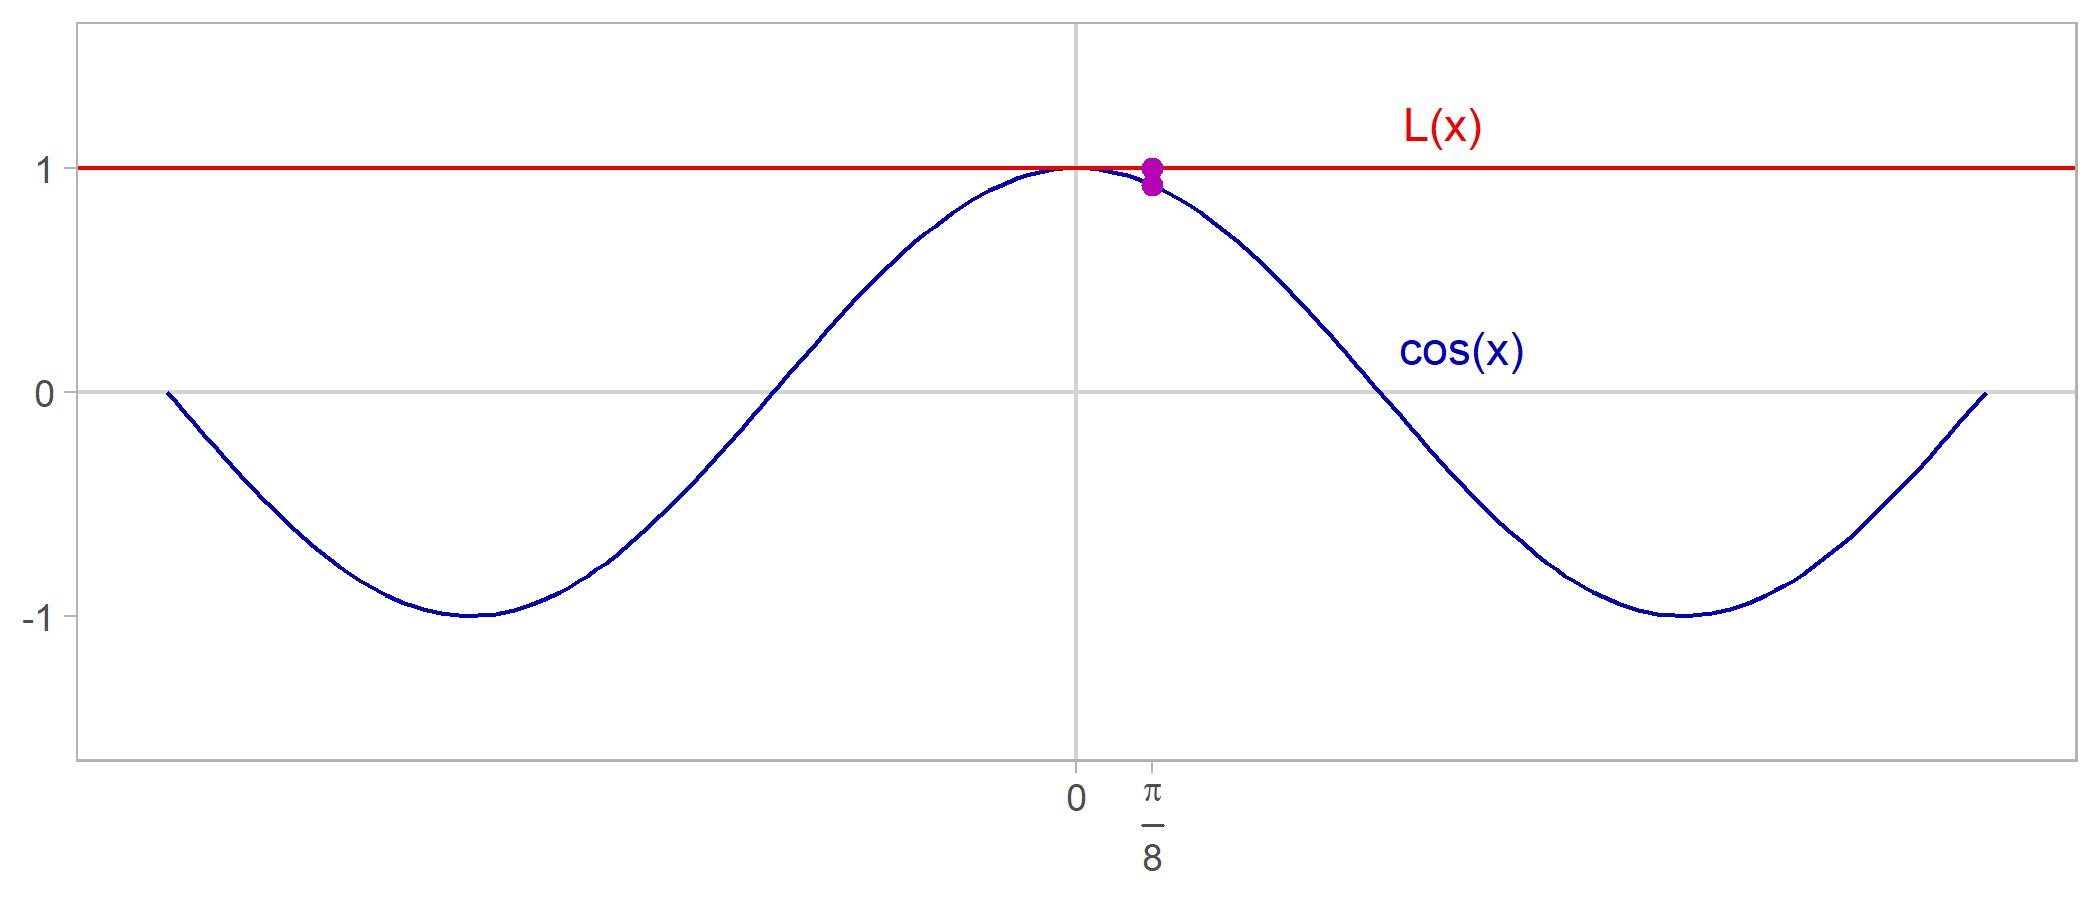
\includegraphics[scale=0.7]{img/quad_approx_1.jpg}
\centering
\end{figure}

Sin embargo, si nos alejamos horizontalmente en solo unos pocos puntos, $L(x)$ comienza a ser mucho menos precisa de lo que era cerca de $x = 0$.

Por ejemplo, en $x = \frac{3\pi}{7}$, $L(x)$ sigue siendo 1, pero usando calculadora, $\cos\left(\frac{3\pi}{7}\right) \approx 0.22252$.

\begin{figure}[hbt!]
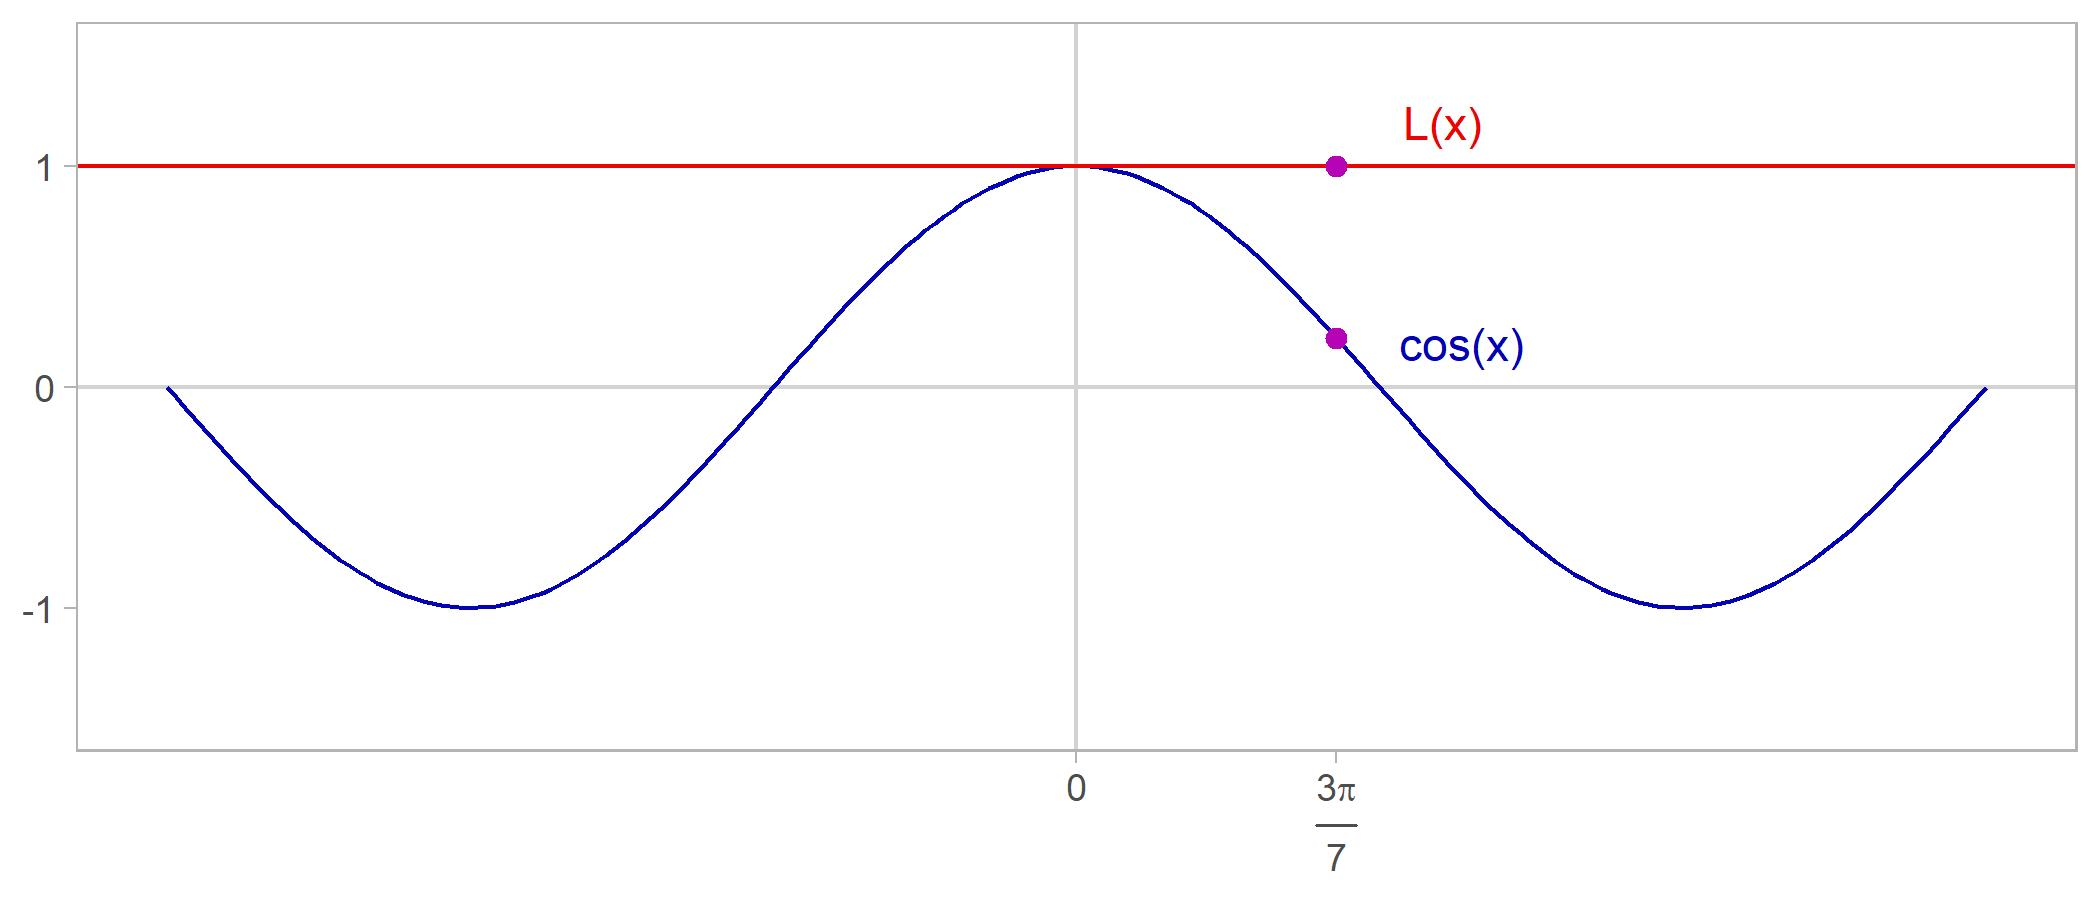
\includegraphics[scale=0.7]{img/quad_approx_2.jpg}
\centering
\end{figure}

Como vemos, la sobreestimación se hace bastante mayor.

Este problema suele darse porque las funciones, en general, suelen ser más curvadas que lineales. Sobre todo si éstas son más complejas y con muchas curvas, se hace más complejo obtener una estimación más precisa usando la aproximación de la línea tangente.

Una forma de resolver este asunto, es aproximarnos usando una \textbf{parábola}, pero debe ser una que \textbf{se ajuste bien a la curvatura de la función}. Por lo tanto, vamos a necesitar información sobre su \textbf{concavidad en un punto} y aquello lo podemos saber a partir de su \textbf{segunda derivada}.

Entonces, digamos que $q(x)$ es la ecuación de una parábola de la forma $a + bx + cx^{2}$; y que $f(x)$ es una función derivable.

El objetivo es que $q(x)$ sea la \textbf{parábola de mejor ajuste} de $f(x)$ en un punto $x = a$. Para ésto, tendrá que cumplirse que:
\[q(a) = f(a) \qquad q'(a) = f'(a) \qquad q''(a) = f''(a)\]
 
Una estrategia que podemos tomar, es usar la fórmula de la aproximación lineal y convertirla en un polinomio de segundo grado agregándole un término cuadrático\footnote{Esto tiene sentido, ya que si $a = 0$, la ecuación se convierte en el polinomio de segundo grado.}:
\[q(x) = f(a) + f'(a)(x - a) + c(x - a)^{2}\]
Ahora, lo que necesitamos es encontrar un valor de $c$ tal que $q''(a) = f''(a)$. Partamos calculando la segunda derivada de $q(x)$.
\[q'(x) = f'(a) + 2cx\]
\[q''(x) = 2c\]
Finalmente, necesitamos que $q''(a) = f''(a)$ y como $q''(x)$ es una función constante, entonces $q''(a) = 2c$. Por lo tanto:
\[2c = f''(a)\]
\[c = \frac{f''(a)}{2}\]
Insertemos el valor $c$ en la fórmula de $q(x)$.
\[q(x) = f(a) + f'(a)(x - a) + \frac{f''(a)}{2}(x - a)^{2}\]
Veamos si se cumple que $q(a) = f(a)$, $q'(a) = f'(a)$ y que $q''(a) = f''(a)$.
\[q(a) = f(a) + f'(a)(a - a) + \frac{f''(a)}{2}(a - a)^{2}\]
\[q(a) = f(a)\]
Se cumple la primera condición. Vayamos por la segunda.
\[q'(x) = f'(a) + f''(a)(x - a)\]
\[q'(a) = f'(a) + f''(a)(a - a)\]
\[q'(a) = f'(a)\]
También se cumple. Veamos si ocurre lo mismo con la segunda derivada.
\[q''(x) = f''(a)\]
\[q''(a) = f''(a)\]
También la segunda derivada de $q(x)$ es igual a la segunda derivada de $f(x)$ en $x = a$.

Por lo tanto, $q(x)$ es la \textbf{parábola de mejor ajuste} de $f(x)$ en $x = a$ y su fórmula corresponde a la \textbf{aproximación cuadrática de una función en un punto}.
\[f(x) \approx f(a) + f'(a)(x - a) + \frac{f''(a)}{2}(x - a)^{2}\]
Ahora, calculemos la aproximación cuadrática de $\cos(x)$ en $x \approx 0$ para ver si es una medida más precisa para estimar el valor de $\cos\left(\frac{3\pi}{7}\right)$.
\[\cos(x) \approx \cos(0) - \sin(0)x - \frac{\cos(0)}{2}x^{2} = 1 - \frac{x^{2}}{2}\]
Asignemos esta fórmula a $q(x)$ y veamos a qué valor se acerca en $x = \frac{3\pi}{7}$.
\[q(x) = 1 - \frac{1}{2} \left(\frac{3\pi}{7}\right)^{2} \approx 0.0936\]
Recordemos que, usando calculadora, $\cos\left(\frac{3\pi}{7}\right) \approx 0.22252$, así que la aproximación cuadrática que acabamos de obtener es una mejor estimación que la calculada anteriormente. 

También podemos observarlo de forma gráfica:

\begin{figure}[hbt!]
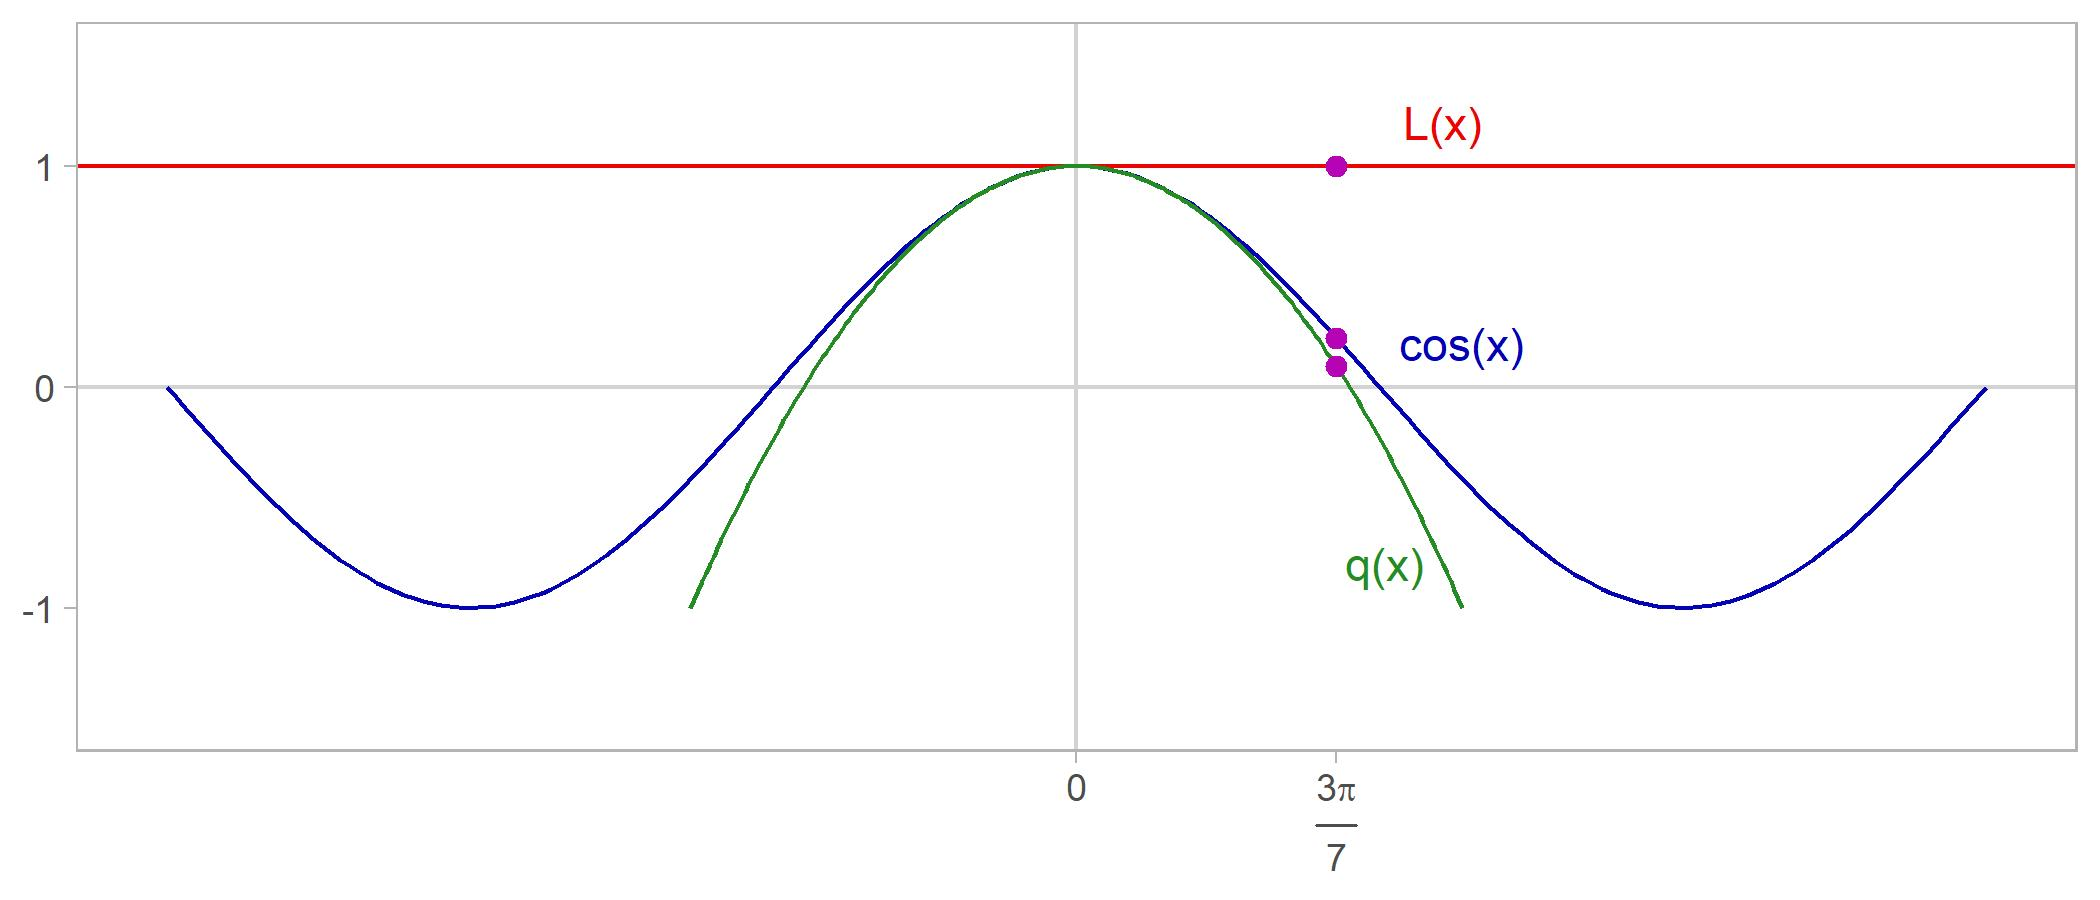
\includegraphics[scale=0.7]{img/quad_approx_3.jpg}
\centering
\end{figure}

\newpage

\subsubsection{Aproximaciones Cuadráticas en $x \approx 0$.}

La aproximación cuadrática de una función $f(x)$ en $x \approx 0$, es la siguiente:
\[f(x) \approx f(0) + f'(0)x + \frac{f''(0)}{2} x^{2}\]
Tal como lo hicimos con la aproximación lineal, calculemos la aproximación cuadrática en $x \approx 0$ de funciones que ya sabemos cómo derivar: $(1 + x)^{r}$, $\sin(x)$, $\cos(x)$, $e^{x}$, $\ln(1 + x)$.

Recordemos que una parte de la aproximación cuadrática, es la fórmula de la aproximación lineal:
\[f(x) \approx \overbrace{f(0) + f'(0)x}^{\text{Appróx. Lineal}} + \frac{f''(0)}{2} x^{2}\]
Por lo tanto, podemos adelantarnos en el cálculo de las aproximaciones cuadráticas cerca de $x = 0$ de las funciones de arriba, puesto que ya conocemos sus aproximaciones lineales en el mismo punto (pág. 10), así que solo tenemos que concentrarnos en sus segundas derivadas.
\[(1 + x)^{r} \approx 1 + rx + \frac{r(r - 1)}{2}x^{2}\]
\[\sin(x) \approx x\]
\[\cos(x) \approx 1 - \frac{x^{2}}{2}\]
\[e^{x} \approx 1 + x + \frac{x^{2}}{2}\]
\[\ln(1 + x) \approx x - \frac{x^{2}}{2}\]

\subsubsection{Producto de Aproximaciones Cuadráticas.}

En ciertos casos, algunas funciones pueden ser el resultado de una operación aritmética entre ella u otras distintas.

Si queremos tomar la \textbf{aproximación cuadrática} de una función de estas características en un punto y nos damos cuenta que corresponde a un \textbf{producto de funciones}, podemos seguir los siguientes pasos:

\begin{enumerate}
\item Calcular la aproximación cuadrática de cada función, por separado, en el mismo punto.

\item Multiplicar las aproximaciones cuadráticas de cada función.

\item Calcular la aproximación cuadrática del producto resultante.
\end{enumerate}

\underline{Ejemplo}: Sean $f(x) = e^{x}$ y $g(x) = \sin(x)$, calcule la aproximación cuadrática de $h(x) = f(x) \cdot g(x)$ cerca de $x = 0$.

\underline{Respuesta}: El primer paso, es calcular las aproximaciones cuadráticas de $f(x)$ y $g(x)$ cerca de $x = 0$, las cuales acabamos de ver.
\[e^{x} \approx 1 + x + \frac{x^{2}}{2} \ \qquad \sin(x) \approx x\]
Luego, multipliquemos estas aproximaciones cuadráticas:
\[\left(1 + x + \frac{x^{2}}{2}\right) \cdot x = x + x^{2} + \frac{x^{3}}{2}\]
Finalmente, como estamos buscando la aproximación cuadrática de esta función, solo tenemos que eliminar los términos superiores al cuadrático. Por lo tanto, la aproximación cuadrática de $h(x)$ en $x \approx 0$, es:
\[h(x) \approx x + x^{2}\]

\underline{Ejemplo}: Calcule la aproximación cuadrática de $f(x) = e^{x + x^{2}}$ cerca de $x = 0$.

\underline{Respuesta}: Una forma para resolver este ejemplo, es aplicar la fórmula de la aproximación cuadrática, pero si nos damos cuenta $f(x) = e^{x} \cdot e^{x^{2}}$, de manera que también podemos usar los pasos de este tipo de aproximación para un producto de funciones. Acá usaremos este camino.

La aproximación cuadrática de $e^{x}$ en $x \approx 0$ ya la conocemos, así que concentrémonos en la de $e^{x^{2}}$.

Partamos con la derivada de $e^{x^{2}}$.
\[\frac{d}{dx} e^{x^{2}} = \frac{d}{dx^{2}} e^{x^{2}} \cdot \frac{d}{dx} x^{2} = 2xe^{x^{2}}\]
Luego, con su segunda derivada:
\[\frac{d}{dx} 2xe^{x^{2}} = 2 \cdot (e^{x^{2}} + 2x^{2}e^{x^{2}})\]
Ahora, calculemos su aproximación cuadrática en $x = 0$.
\[e^{x^{2}} \approx e^{0^{2}} + \left(2 \cdot 0 \cdot e^{0^{2}}\right)x + \frac{2 \cdot (e^{0^{2}} + (2 \cdot 0^{2} \cdot e^{0^{2}}))}{2} x^{2} = 1 + x^{2}\]
Finalmente, multiplicamos las aproximaciones cuadráticas de $e^{x}$ y $e^{x^{2}}$; y eliminamos los términos que son superiores al cuadrático para obtener la aproximación cuadrática de $f(x)$ en $x \approx 0$.
\[f(x) \approx \left(1 + x + \frac{x^{2}}{2}\right) \cdot (1 + x^{2}) = 1 + x + \frac{x^{2}}{2} + x^{2} + x^{3} + \frac{x^{4}}{2}\]
\[f(x) \approx 1 + x + \frac{3}{2} x^{2}\]


\subsubsection{Notación ``$\mathcal{O}$ Grande''.}

Las aproximaciones lineal (1) y cuadrática (2) de $(1 + x)^{5}$ cerca de $x = 0$, son las siguientes:
\[
\text{(1) } (1 + x)^{5} \approx 1 + 5x
 \qquad \qquad 
\text{(2) } (1 + x)^{5} \approx 1 + 5x + 10x^{2}
\]
Una duda que puede surgirnos es \textbf{a qué nos referimos con que se ``aproximen'' a dichas expresiones} o, dicho de otro modo, qué significa exactamente el símbolo ``$\approx$''.

El que nos ``aproximemos'' quiere decir que la función es igual a una expresión \textbf{más un término de error}. Es decir, válido señalar que:
\[
\text{(1) } (1 + x)^{5} = 1 + 5x + \text{error}
 \qquad \qquad 
\text{(2) } (1 + x)^{5} = 1 + 5x + 10x^{2} + \text{error}
\]
Donde el término de error de la aproximación lineal \textbf{no es el mismo} al de la aproximación cuadrática. Esto significa que hay una forma para \textbf{medir el tamaño de estos errores}, lo que nos permitiría \textbf{conocer el nivel precisión} de estas aproximaciones. En otras palabras, el \textbf{orden de magnitud} de estos términos.

Por ejemplo, ya sabemos que la aproximación cuadrática de una función es más precisa que su aproximación lineal\footnote{Ver como ejemplo la gráfica de la pág. 22.}, pero hasta ahora no tenemos una forma de medir cuantitativamente aquello y eso es lo que veremos a continuación.

Algo a dejar en claro es que \textbf{no buscaremos el valor exacto de los términos de error}, sino que solo veremos una forma de cuantificar la magnitud o el nivel de incidencia de éstos.

Concentrémonos en la \textbf{aproximación lineal} de $(1 + x)^{5}$ \textbf{cerca de} $x = 0$.

%\newpage

Si expandimos el polinomio $(1 + x)^{5}$, obtendremos que:
\[(1 + x)^{5} = 1 + 5x + 10x^{2} + 10x^{3} + 5x^{4} + x^{5}\]
\newpage
En la \textbf{aproximación lineal}, el término de error es la expresión que va posterior a la parte lineal de esta función.
\[\text{error} = 10x^{2} + 10x^{3} + 5x^{4} + x^{5}\]
Por otra parte, no olvidemos que es la \textbf{aproximación lineal cercano a cero}, lo que implica que, \textbf{mientras más grande sean los valores de los exponentes, más chico será su valor}.

Por ejemplo, si $x = 0.1$, entonces:

\begin{table}[hbt!]
\begin{tabular}{c | c c c c}
$x$ & $x^{2}$ & $x^{3}$ & $x^{4}$ & $x^{5}$ \\
\hline
0.1 & 0.01 & 0.001 & 0.0001 & 0.00001 \\
\end{tabular}
\centering
\end{table}

Como vemos en la tabla de arriba, a nivel de magnitud, el término que más incidirá en el error de la aproximación lineal en $x \approx 0$ de $(1 + x)^{5}$, es $x^{2}$, mientras que $x^{4}$ y $x^{5}$ son los que generan menos efecto.

El \textbf{término de error} lo vamos a entender como un \textbf{valor límite}. Es decir, será menor o igual a un número en función del término más relevante.

Entonces, veamos cuál es el tamaño del término de error cuando $|x| < 0.1$.

Para hacer más fácil el cálculo, trabajemos con notación científica y establezcamos que $0.1 = 10^{-1}$. Por lo tanto\footnote{Hay muchas formas de hacer el cálculo de a continuación. Al parecer solo se resuelve intuitivamente, pero decidí hacerlo de esta manera porque lo entendí mejor.}:
%\[|\text{error}| \leq 10(10^{-1})^{2} + 10(10^{-1})^{3} + 5(10^{-1})^{4} + (10^{-1})^{5}\]
\begin{align*}
	|\text{error}| &\leq 10(10^{-1})^{2} + 10(10^{-1})^{3} + 5(10^{-1})^{4} + (10^{-1})^{5} \\
	&\leq 10^{-1} + 10^{-2} + 5 \cdot 10^{-4} + 10^{-5}
\end{align*}
Como $x^{2}$ es el término más determinante en el nivel de error que tendrá la aproximación lineal en $x \approx 0$, lo que haremos es buscar un valor tal que al multiplicarlo por $10^{-2}$ (i.e., $0.1^{2} = x^{2}$) nos de cada uno de los sumandos de arriba.

Por ejemplo, sea $a$ un valor que buscamos, tal que:
\[a \cdot 10^{-2} = 10^{-1}\]
\[a = \frac{10^{-1}}{10^{-2}} = 10\]

\newpage

Por consiguiente, podemos establecer que:
\[|\text{error}| \leq 10x^{2} + 10^{-2} + 5 \cdot 10^{-4} + 10^{-5}\]
Si usamos el mismo método en los demás sumandos del error, obtendremos la siguiente expresión:
\[|\text{error}| \leq 10x^{2} + 10^{0}x^{2} + 5 \cdot 10^{-2}x^{2} + 10^{-3}x^{2}\]
\[|\text{error}| \leq 11.051x^{2}\]
Para asegurarnos que el error esté totalmente considerado, lo redondearemos al entero mayor.
\[|\text{error}| \leq 12x^{2}\]
Entonces, en $|x| < 0.1$, el error en valor absoluto de la aproximación lineal de $(1 + x)^{5}$ en $x \approx 0$, es menor o igual que $12x^2$.

En otras palabras, lo que este valor nos está diciendo es que los términos que vienen después de $1 + 5x$ (i.e., la apróx. lineal) no son mayores a una constante multiplicada por $x^{2}$, cuando $x \to 0$.

Por lo tanto, el \textbf{orden de magnitud} del error en la aproximación lineal, es menor o igual una constante multiplicada por $x^{2}$. Una forma de comúnmente usada para expresar este orden de magnitud, se la conoce como la \textbf{Notación $\mathcal{O}$ Grande}.

Por ejemplo, la aproximación lineal de $(1 + x)^{5}$ en $x \approx 0$, podemos escribirla como:
\[(1 + x)^{5} = 1 + 5x + O(x^{2})\]
Donde $O(x^{2})$ se la lee\footnote{Ojo con esto último, porque \textbf{NO estamos diciendo que $O(x^{2})$ es una función}. Es simplemente una notación.} como ``$\mathcal{O}$ grande de $x^{2}$'' y  nos dice que las expresiones mayores a $x^{2}$, son insignificantes.

Formalmente, a una función $f(x)$ cuyo orden de magnitud es $x^{n}$ cerca de $x = 0$, se la denota como:
\[f(x) = O(x^{n}) \; \text{ en } \; x \approx 0 \quad \text{si} \quad |f(x)| \leq kx^{n} \: \: (k = \text{cte})\]
Donde $f(x) = O(x^{n})$ se lee\footnote{Como vemos, la expresión $f(x) = O(x^{n})$ no es una igualdad o no sugiere que hay una simetría entre $f(x)$ y $O(x^{n})$. Debido a este motivo, algunas personas prefieren denotarlo como $f(x) \in O(x^{n})$. Recomiendo leer esta \href{https://en.wikipedia.org/wiki/Big_O_notation\#Equals_sign}{sección de wikipedia} sobre el signo ``igual'' en la notación $\mathcal{O}$ grande.} como ``$f(x)$ \textbf{es} $\mathcal{O}$ grande de $x^{n}$''.

\newpage

%Como vemos, la expresión $f(x) = O(x^{n})$ no es una igualdad o no sugiere que hay una simetría entre $f(x)$ y $O(x^{n})$. Debido a este motivo, algunas personas prefieren denotarlo como $f(x) \in O(x^{n})$. Recomiendo leer esta \href{https://en.wikipedia.org/wiki/Big_O_notation#Equals_sign}{sección de wikipedia} sobre el signo ``igual'' en la notación $\mathcal{O}$ grande.
%\newpage

%Algunas personas lo denotan como $f(x) = O(x^{n})$, pero el símbolo ``$=$'' no debe leerse como ``igual'', sino como ``es'' (e.g, $f(x) = O(x^{2})$ se lee como ``$f(x)$ \textbf{es} $\mathcal{O}$ grande de $x^{2}$''), porque no es una igualdad o no sugiere una simetría propiamente tal. Recomiendo leer esta \href{https://en.wikipedia.org/wiki/Big_O_notation#Equals_sign}{sección de wikipedia} sobre el signo ``igual'' en la notación $\mathcal{O}$ grande.

%sección de wikipedia
%https://en.wikipedia.org/wiki/Big_O_notation#Equals_sign
%\newpage

Anteriormente vimos cómo escribir la aproximación lineal cerca de $x = 0$ de $(1 + x)^{5}$ considerando el orden de magnitud de su error; y dicha expresión la podemos generalizar.

Para cualquier función continua $f(x)$, \textbf{el orden de magnitud de su aproximación lineal} mientras $x \to 0$, es $O(x^{2})$. Por lo tanto, aquella aproximación también podemos denotarla como:
%Por lo tanto, lo anterior implica que, \textbf{para cualquier función} $f(x)$, el \textbf{error de su aproximación lineal} es $O(x^{2})$. Es decir:
\[f(x) = f(0) + f'(0)x + O(x^{2})\]
Algo similar ocurre con la \textbf{aproximación cuadrática}, pero en este caso el orden de magnitud del error es, $O(x^{3})$. Por consiguiente:
\[f(x) = f(0) + f'(0)x + \frac{f''(0)}{2}x^{2} + O(x^{3})\]
Lo que nos dice que, en la aproximación cuadrática de $f(x)$ en $x \approx 0$, los términos mayores al producto $kx^{3}$, son insignificantes. Serán determinantes solo si son menores o iguales a dicha multiplicación.

\subsubsection{Calculando el Error y la Constante de la Notación $\mathcal{O}$ Grande.}

Volvamos a la función $(1 + x)^{5}$.

Cuando calculamos el error de su aproximación lineal cerca de $x = 0$, establecimos que correspondía a la parte posterior de la aproximación, la cual obtuvimos expandiendo el polinomio de quinto grado. Sin embargo, si hacemos lo mismo con uno más grande (e.g, $(1 + x)^{15}$) sería tedioso usar ese enfoque. Ahora, con la definición de la notación $\mathcal{O}$ grande (pág. 27), podemos hacer ese cálculo más fácil.

A partir de la aproximación lineal de $(1 + x)^{5}$, ya sabemos que
\[(1 + x)^{5} = 1 + 5x + O(x^{2})\]
Por lo tanto, cerca de $x = 0$, la aproximación lineal de $(1 + x)^{5}$ no es mayor a $kx^{2}$, que es la expresión que nos permite cuantificar el error de la aproximación.

Es decir, la distancia entre el valor real de la función y el valor de su aproximación lineal en $x \approx 0$, en un punto $x$, es menor o igual al producto entre una constante y $x^{2}$. Por consiguiente, es válido establecer que:
\[|\text{error}| = |(1 + x)^{5} - (1 + 5x)|\]
Sabemos que $|\text{error}| \leq kx^{2}$, por lo tanto:
\[|(1 + x)^{5} - (1 + 5x)| \leq kx^{2}\]
A partir de esta fórmula, también podemos calcular fácilmente la constante:
\[\frac{|(1 + x)^{5} - (1 + 5x)|}{x^{2}} \leq k\]
Lo cual hace sentido, ya que $k$ depende del valor que tome $x$.

Por ejemplo, cuando vimos que $|x| < 0.1$, obtuvimos que $11.051 \leq k$. Por lo tanto, a medida que $x \to 0$, $k$ se hará más irrelevante y solo $x^{2}$ será determinante en la aproximación lineal de $(1 + x)^{5}$. Dicho de otro modo, su orden de magnitud será $x^{2}$.

Entonces, sea $f(x)$ una función continua, el error de su aproximación lineal mientras $x \approx 0$ es:
\[|f(x) - (1 + f'(0)x)| \leq kx^{2}\]
Mientras que el error de la aproximación cuadrática, a medida que $x \approx 0$, es:
\[\left|f(x) - \left(1 + f'(0)x + \frac{f''(0)}{2} x^{2}\right)\right| \leq kx^{3}\]

\underline{Ejercicio}: Suponga que pide un préstamo de \$15000 para comprarse un auto, cuya tasa de interés es de 3\% por año, compuesto mensualmente.

La cantidad de interés acumulado (\textit{amount of interest accrued}) durante un período de tiempo $T$ medido en meses, se puede calcular usando la siguiente fórmula:
\[A = 15000\left(1 + \frac{0.03}{12}\right)^{T} - 15000\]
A partir de la información dada, responda las siguientes preguntas:

\begin{itemize}
\item[(a)] Use la aproximación cuadrática para calcular la cantidad de interés acumulado aproximado en 4 años.

\item[(b)] Calcule el término de error exacto de la aproximación cuadrática.

\item[(c)] Utilice el error calculado para obtener el orden de magnitud de $k$.
\end{itemize}

\newpage

\underline{Respuesta (a)}: En la fórmula de la cantidad de interés acumulado ($A$), tenemos un término de la forma $(1 + x)^{r}$, donde el exponente es un valor fijo. Podemos usarla para calcular la aproximación cuadrática de $A$ a medida que $x \to 0$.

En este caso, diremos que $x = 0.03/12$, ya que es la tasa de interés y ésta varía en un período de tiempo.

En cuanto a $T$, como son 4 años y se miden en meses, entonces $T = 12 \cdot 4 = 48$ meses.

Por lo tanto:
\begin{align*}
A &\approx
	15000\left(1 + 48x + \frac{48(47)}{2} x^{2} \right) - 15000 \\
  &\approx 15000(1 + 48x + 1128 x^{2}) - 15000
\end{align*}
Factoricemos por 15000 para hacer más fácil el cálculo:
\[
A \approx 15000(48x + 1128x^{2})
\]
Finalmente, reemplacemos $x$ para conseguir el valor aproximado de $A$ en un periodo de 4 años.
\begin{align*}
A &\approx 15000 \left[48 \left(\frac{0.03}{12}\right) +
		   1128 \left(\frac{0.03}{12}\right)^{2}\right] \\
  &\approx 1905.75
\end{align*}
Por lo tanto, la cantidad de interés acumulado en 4 años, es de \$1905.75, aproximadamente.

\underline{Respuesta (b)}: Ahora, cuantifiquemos el error de la aproximación cuadrática que acabamos de calcular.

Como es una aproximación cuadrática cerca de $x = 0$, entonces $A = O(x^{3})$. Es decir, el valor real de $A$ no es mayor a una constante multiplicada por $x^{3}$.

Recordemos que el error lo calculamos como la diferencia entre el valor real y su aproximación, a medida que $x \to 0$, donde $x = 0.03/12$. Por lo tanto:
\[
\left|\left(1 + \frac{0.03}{12}\right)^{48} - 1905.75\right|
	\leq kx^{3}
\]
Usando calculadora, obtenemos que el error es:
\[4.17 ... \leq kx^{3}\]

\underline{Respuesta (c)}: Para terminar, veamos cuál es el orden de magnitud de la constante $k$ del error de la aproximación cuadrática.

Para ello, usemos la expresión con la que terminamos en la parte (b) del ejemplo y despejemos $k$, considerando que $x = 0.03/12$.
\[k \geq \frac{4.17 ...}{(0.03/12)^{3}}\]
Con calculadora, el resultado de $k$ es el siguiente:
\[k \geq 266900198.33...\]
El orden de magnitud es, simplemente, pasar este resultado a notación científica y ver a qué exponente se eleva el múltiplo de 10.
\[k \geq 2.6690019833... \cdot 10^{8}\]
Por consiguiente, el orden de magnitud\footnote{En el ejercicio, la respuesta es $10^{8}$, pero en la mayoría de los lugares en donde busqué información, se hacía referencia al orden de magnitud como el valor del exponente de la potencia de base 10. Así que acá preferí responder de esta otra forma.} de $k$ es 8.

\subsubsection{Notación $\mathcal{O}$ grande y Funciones Complicadas.}

Veamos cómo se vincula la aproximación cuadrática en $x \approx 0$ y la notación $\mathcal{O}$ en funciones más complicadas.

\underline{Ejemplo}: Calcule la aproximación cuadrática cerca de $x = 0$ de $e^{\sin(x)}$.

\underline{Respuesta}: Podemos partir calculando la aproximación cuadrática de $\sin(x)$ y establecer que:
\[e^{\sin(x)} = e^{x + O(x^{3})}\]
Es posible establecer esta igualdad, porque estamos considerando $O(x^{3})$ en la aproximación.

\newpage

Luego, definamos que $u = 1 + O(x^{3})$ para poder calcular más fácilmente la aproximación cuadrática de $e^{x + O(x^{3})}$.
\[e^{u} = 1 + u + \frac{1}{2}u^{2} + O(u^{3})\]
Reemplacemos $u$ por su expresión original.
\[
e^{x + O(x^{3})} = 1 + x + O(x^{3}) + \frac{1}{2} (x + O(x^{3}))^{2}
                   + O\left((x + O(x^{3}))^3\right)
\]
En la expresión de arriba tenemos un binomio cuadrático y otro cúbico, los cuales involucra a $O(x^{3})$. Lo que haremos es resolverlos, pero cualquier término mayor a $x^{3}$ lo reemplazaremos por $O(x^{3})$, sea un exponente mayor a 3 o una constante que esté multiplicando a $x^{3}$ o a $O(x^{3})$.

Resolvamos ambos binomios de forma separada, para mayor legibilidad.
\begin{align*}
\frac{1}{2} (x + O(x^{3}))^{2} &=
	\frac{1}{2} (x^{2} + 2xO(x^{3}) + (O(x^{3}))^{2}) \\
 &= \frac{1}{2}x^{2} + \frac{1}{2}O(x^{3}) \\
 & = \frac{1}{2} x^{2} + O(x^{3})
\end{align*}
Las constantes o cualquier valor que rodee a $O(x^{3})$ las sacamos porque, a medida que $x \to 0$, $x^{3}$ será la única expresión relevante de la aproximación cuadrática.

Veamos ahora el cubo del binomio.
\begin{align*}
O\left((x + O(x^{3}))^3\right) &=
	O(x^{3} + 3x^{2}O(x^{3}) + 3x(O(x^{3}))^{2} + (O(x^{3}))^{3}) \\
  &= O(x^{3})
\end{align*}
En este caso, solo $x^{3}$ es el término relevante.

Finalmente, reemplacemos el cuadrado y el cubo de los binomios en la aproximación cuadrática.
\[
e^{x + O(x^{3})} = 1 + x + O(x^{3})
                   + \frac{1}{2} x^{2} + O(x^{3})
                   + O(x^{3})
\]
Al sumar los $O(x^{3})$ obtendremos $3O(x^{3})$, pero sabemos que cerca de $x = 0$ las constantes se vuelven insignificantes, así que podemos dejar esta expresión como $O(x^{3})$.

Por lo tanto, la expresión final de la aproximación cuadrática es la siguiente:
\[e^{\sin(x)} = 1 + x + \frac{1}{2} x^{2} + O(x^{3})\]

\newpage

Veamos otro ejemplo.

\underline{Ejemplo}: Calcule la aproximación cuadrática cerca de $x = 0$ de $e^{-3x}/\sqrt{1 + x}$.

\underline{Respuesta}: La expresión $e^{-3x}/\sqrt{1 + x}$ es posible denotarla también como:
\[\frac{e^{-3x}}{\sqrt{1 + x}} = e^{-3x} \cdot (1 + x)^{-1/2}\]
No olvidemos que, cuando nos encontramos con funciones más complicadas como la de este ejemplo y queremos tomar su aproximación cuadrática (o lineal, también), lo mejor es trabajarlas como productos si es que tenemos aquella posibilidad.

Luego, tomemos sus aproximaciones cuadráticas por separado y considerando $O(x^{3})$.

Como ya sabemos que cualquier término mayor a $x^{3}$ es insignificante cerca de $x = 0$, estableceremos de inmediato que dicha parte es $O(x^{3})$, para hacer más rápido el cálculo a cómo lo hicimos en el ejemplo anterior.
\begin{align*}
\frac{e^{-3x}}{\sqrt{1 + x}} &=
	\left(1 - 3x + \frac{9}{2}x^{2} + O(x^{3})\right) \cdot
	\left(1 - \frac{1}{2}x + \frac{3}{8}x^{2} + O(x^{3})\right) \\
 &= 1 - \frac{1}{2}x - 3x + \frac{3}{8}x^{2} + \frac{3}{2}x^{2}
    + \frac{9}{2}x^{2} + O(x^{3}) \\
\frac{e^{-3x}}{\sqrt{1 + x}} &= 1 - \frac{7}{2}x
                                + \frac{51}{8}x^{2} + O(x^{3})
\end{align*}



\subsection{Método de Newton.}

La aproximación lineal también puede ser usada para \textbf{obtener los ceros o raíces de una función real}. Es decir, ver en qué valor(es) se iguala a cero o, geométricamente, en qué punto la curva intersecta al eje X.

Muchas veces nos encontraremos con que el cero de la función corresponde a un número irracional. Acá usaremos la \textbf{aproximación lineal} de dicha función de \textbf{forma repetida} para acercarnos casi exactamente al valor real.

Usemos la función $f(x) = 2 - x^{2}$ como ejemplo, cuya gráfica es la siguiente:

\newpage

\begin{figure}[hbt!]
\centering
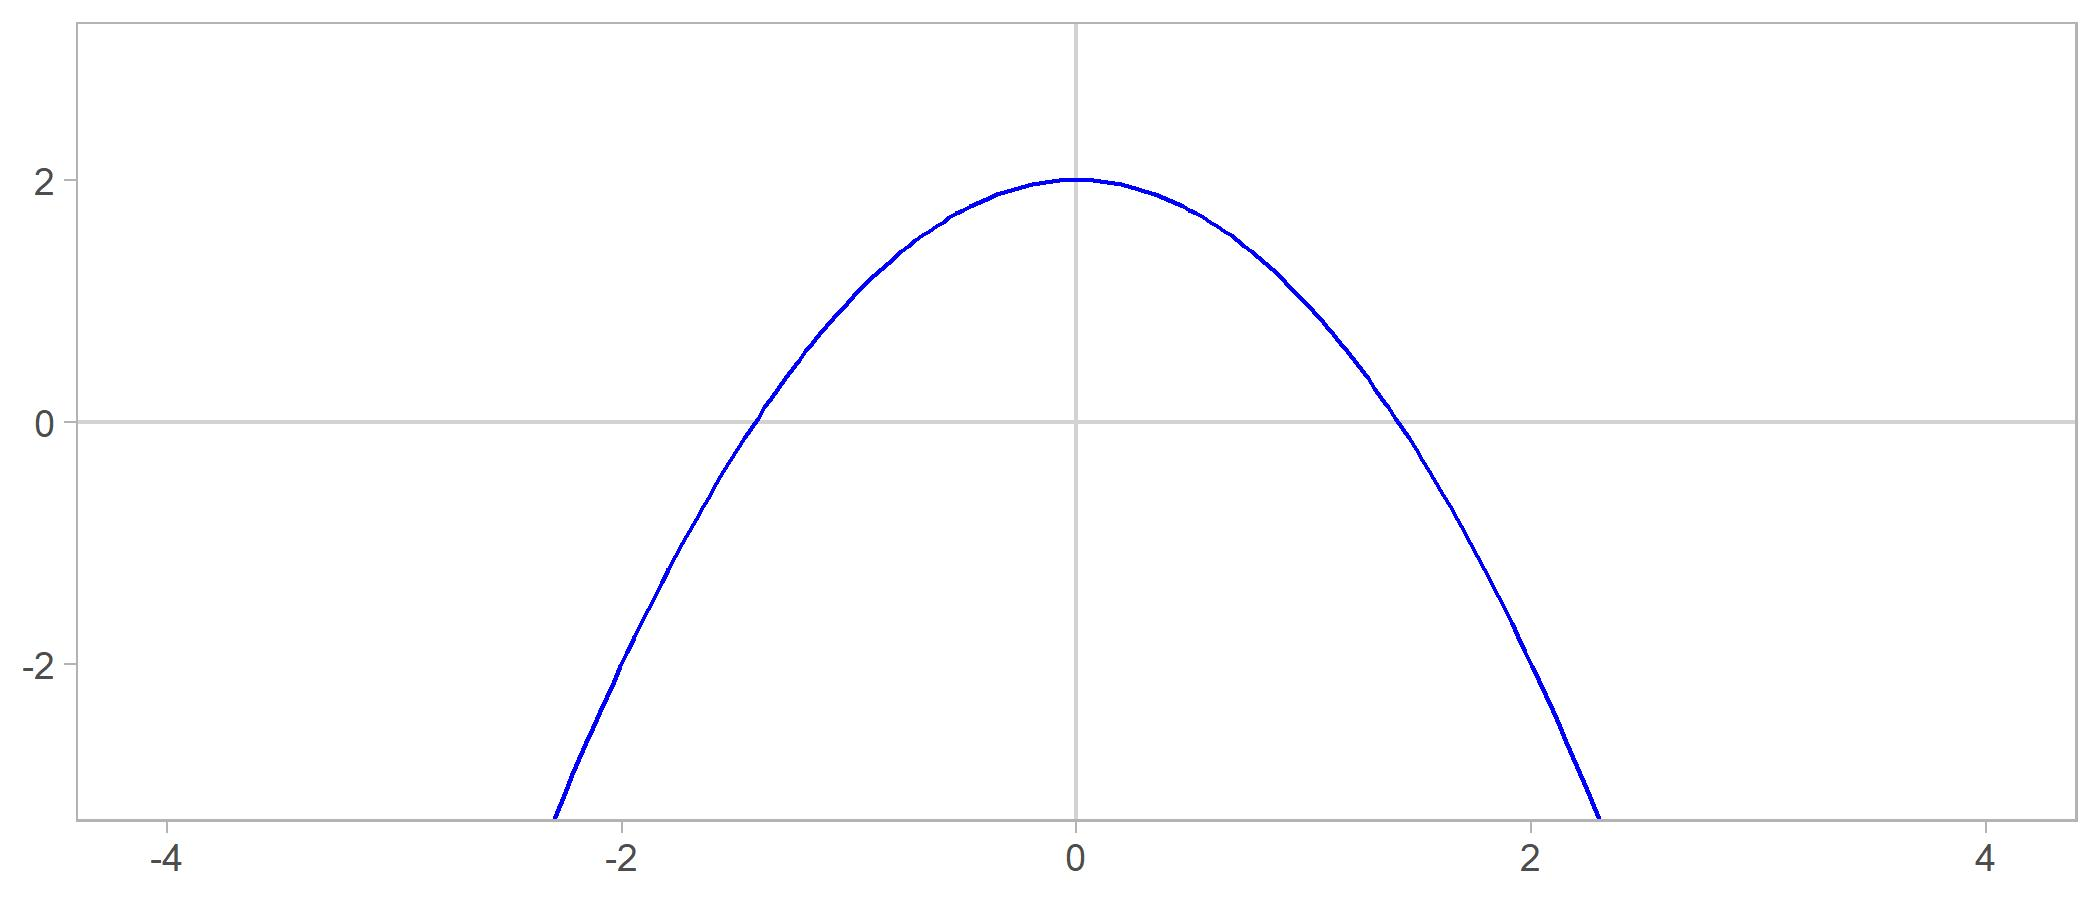
\includegraphics[scale=0.7]{img/newton_general_plot.jpg}
\end{figure}

Los ceros de $f(x)$ podemos encontrarlos igualándola a cero o usando la fórmula cuadrática\footnote{Fórmula cuadrática: \[x = \frac{-b \pm \sqrt{b^{2} - 4ac}}{2a}\]}.
\begin{align*}
0 &= 2 - x^{2} & x &= \frac{0 \pm \sqrt{0^{2} - 4(-1)(2)}}{-2} \\
\pm \sqrt{2} &= x & x &= \pm \sqrt{2}
\end{align*}
Entonces, cuando $x = \pm\sqrt{2}$, $f(x) = 0$.

En este ejemplo, centrémonos solo en $x = \sqrt{2}$.

Usando calculadora, veremos que $\sqrt{2} \approx 1.414214$. La idea es \textbf{usar la aproximación lineal} de $f(x)$ en un punto, \textbf{definirla como una función lineal y buscar el cero de ésta}. Como aún estaremos algo alejados del valor real, volveremos a realizar este procedimiento, pero calcularemos la aproximación lineal cerca del cero que obtuvimos anteriormente. \textbf{Al repetir este método muchas veces, vamos a notar que iremos convergiendo al valor real de} $\sqrt{2}$.

Como vamos a calcular la aproximación lineal de $f(x)$, antes tenemos que conocer la derivada de esta función.
\[\frac{d}{dx} (2 - x^{2}) = -2x\]
Ahora, comencemos calculando la aproximación lineal de $f(x)$ cerca de $x_{0} = 1$, la cual la definiremos como $L(x)$.
\begin{align*}
L(x) &= (2 - (1)^{2}) + (-2(1))(x - 1) \\
     &= 3 - 2x
\end{align*}

\newpage

Busquemos el cero de $L(x)$.
\begin{align*}
0 &= 3 - 2x \\
1.5 &= x
\end{align*}
Entonces, la aproximación lineal de $f(x)$ en $x_{0} \approx 1$ corta al eje X en el punto $x = 1.5$, el cual es cercano al valor de $\sqrt{2}$, pero podríamos precisarlo más. Para ello, volvamos a realizar este procedimiento, pero cerca de $x_{1} = 1.5$.
\begin{align*}
L(x) &= (2 - (1.5)^{2}) + (-2(1.5))(x - 1.5) \\
     &= \frac{17}{4} - 3x
\end{align*}
Luego, sigamos con la raíz o el cero de $L(x)$.
\begin{align*}
0 &= \frac{17}{4} - 3x \\
x &= \frac{17}{12} = 1.41\bar{6}
\end{align*}
Como vemos, ahora nos acercamos más al valor real de $\sqrt{2}$. Volvamos a hacerlo una vez más, pero igualemos a cero de inmediato la aproximación lineal, para hacer más rápido el cálculo.
\begin{align*}
0 &= \left(2 - \left(\frac{17}{12}\right)^{2}\right)
     + \left(-2 \cdot \frac{17}{12}\right)
     \left(x - \frac{17}{12}\right) \\
0 &= \frac{577}{144} - \frac{17}{6}x \\
x &= \frac{577}{408} \approx 1.41422
\end{align*}
La aproximación lineal está mucho más cerca de $\sqrt{2}$. Veamos esta convergencia en la siguiente visualización.

\newpage

\begin{figure}[hbt!]
\centering
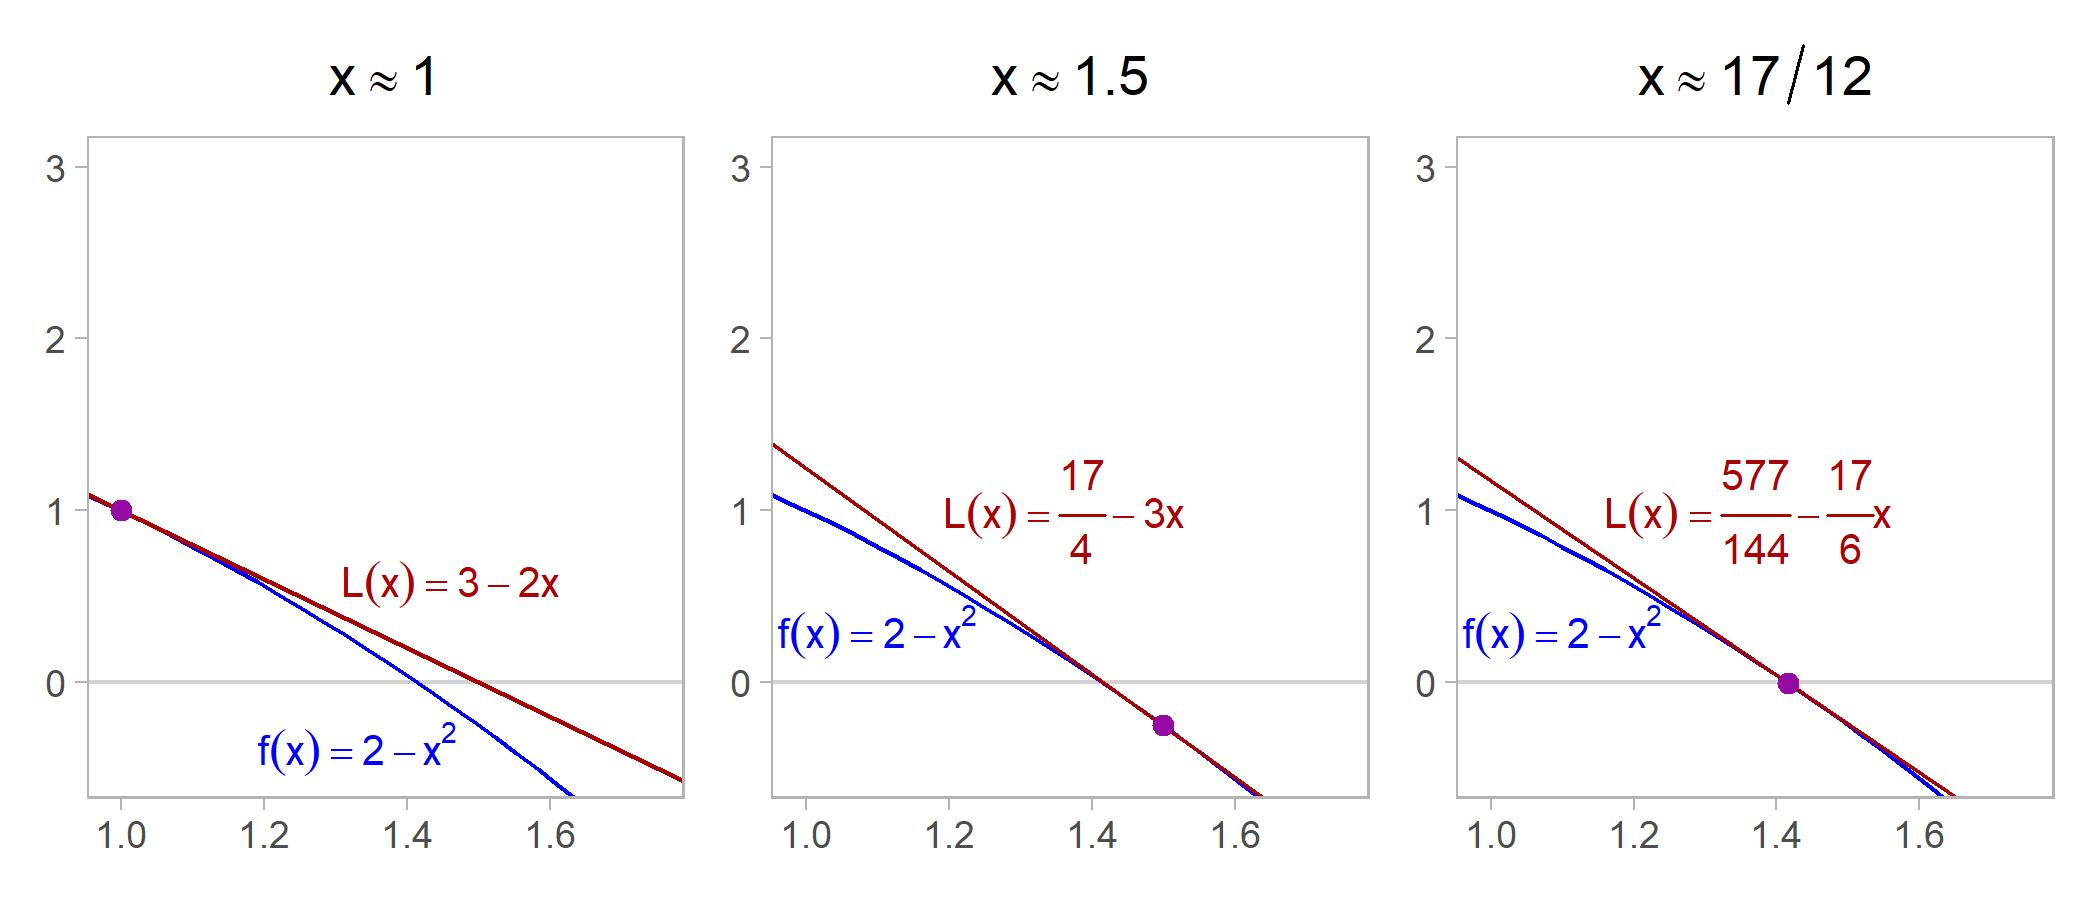
\includegraphics[scale=0.7]{img/newton_and_approx.jpg}
\end{figure}

En la imagen de arriba se puede observar cómo la línea que corresponde a la aproximación lineal de $f(x) = 2 - x^{2}$ (color rojo) se va acercando al cero de esta función, a medida que la vamos calculando a partir del punto de intersección con el eje X que obtuvimos de la anterior.

Lo que acabamos de realizar se llama \textbf{``Método de Newton''} o método de Newton-Raphson, el cual corresponde a un \textbf{algoritmo\footnote{Una secuencia finita y bien definida de instrucciones.} para encontrar aproximaciones de los ceros o raíces de una función real}.

Los pasos del método de Newton, son los siguientes:

\begin{enumerate}
\item Elegir un valor $x_{0}$ como nuestra apuesta aproximada al valor de la raíz de $f(x)$.

\item Buscar el punto $x_{1}$ donde la línea tangente de $f(x)$ en $x_{0}$ intersecte al eje X.
\begin{align*}
0 &= f(x_{0}) + f'(x_{0})(x_{1} - x_{0}) \\
x_{1} &= x_{0} - \frac{f(x_{0})}{f'(x_{0})}
\end{align*}
\item Repetir paso 2, pero con los puntos $x_{1}$ y $x_{2}$.
\[
	x_{2} = x_{1} - \frac{f(x_{1})}{f'(x_{1})}
\]
\end{enumerate}

El paso 2 podemos repetirlos muchas veces. Por lo tanto, en términos generales decimos que:

\newpage

\[x_{n + 1} = x_{n} - \frac{f(x_{n})}{f'(x_{n})}\]
Donde $x_{n + 1}$ es la \textbf{aproximación a la raíz de $f(x)$}.


\subsubsection{Tasa de Convergencia del Método de Newton.}

A partir de lo que hemos aprendido sobre la aproximación lineal y la notación $\mathcal{O}$ grande, podemos entender qué tan rápido converge el método de Newton, comprendiendo el orden de magnitud de los términos de error posteriores a la primera aproximación de la raíz de una función.

Por ejemplo, digamos que $f(x)$ es una función real y que $x^{*}$ es su raíz. Esto implica que $f(x^{*}) = 0$.

Vamos a intentar aproximarnos a la raíz de $f(x)$ usando el método de Newton. Por lo tanto, comenzaremos apostando a que este valor se aproxima a $x_{0}$.

Como $x_{0}$ es una aproximación, consideraremos su tasa de error como la diferencia entre éste y la raíz $x^{*}$, al cual denotaremos como $\varepsilon_{0}$.
\[\varepsilon_{0} = x^{*} - x_{0}\]
Luego, volvemos a hacer el mismo proceso, pero nuestra aproximación a $x^{*}$ será $x_{1}$. En consecuencia su error, $\varepsilon_{1}$, será:
\[
\varepsilon_{1} = x^{*} - x_{1}
	\qquad \text{donde} \qquad
x_{1} = x_{0} - \frac{f(x_{0})}{f'(x_{0})}
\]
Ahora, tratemos de ver cuál es el orden de magnitud de $\varepsilon_{1}$. Para ello, usaremos la aproximación lineal\footnote{Quizá pueda confundirnos un poco que usemos la $O((x - x_{0})^{2})$, ya que antes la denotábamos como $O(x^{2})$, pero recordemos que aquello se debía a que la aproximación lineal la tomábamos cerca de $x = 0$. Ahora es cerca de una expresión $x_{0}$.} de $f(x)$ cerca de $x = x_{0}$.
\[
	f(x) = f(x_{0}) + f'(x_{0})(x - x_{0}) + O((x - x_{0})^{2})
\]
Posteriormente, establezcamos que $x = x^{*}$, la raíz de $f(x)$.
\[
	f(x^{*}) = f(x_{0}) + f'(x_{0})(x^{*} - x_{0})
	           + O((x^{*} - x_{0})^{2})
\]

\newpage

Sabemos que $f(x^{*}) = 0$ y que $\varepsilon_{0} = x^{*} - x_{0}$. Por lo tanto:
\[
	0 = f(x_{0}) + f'(x_{0})\varepsilon_{0} + O(\varepsilon_{0}^{2})
\]
Si resolvemos\footnote{Recordemos que la $O(\varepsilon_{0}^{2})$ se mantendrá positiva, porque cualquier constante que la rodee será insignificante al valor que tome la función, a medida que se acerca a $x_{0}$.} esta ecuación para $f(x_{0})$, obtendremos que:
\[
 f(x_{0}) = - f'(x_{0})\varepsilon_{0} + O(\varepsilon_{0}^{2})
\]
Volvamos a la ecuación del error $\varepsilon_{1}$.
\[\varepsilon_{1} = x^{*} - x_{1}\]
Sabemos que, por el método de Newton, $x_{1}$ corresponderá a:
\[
\varepsilon_{1} = x^{*}
                  - \left[x_{0} - \frac{f(x_{0})}{f'(x_{0})}\right]
\]
Por otra parte, vimos que $f(x_{0}) = - f'(x_{0})\varepsilon_{0} + O(\varepsilon_{0}^{2})$. Por consiguiente:
\begin{align*}
% Quedó desordenado, lo sé :c
\varepsilon_{1} &= x^{*}
                  - \left[
                      x_{0} -
                      \frac{- f'(x_{0})\varepsilon_{0} +
                            O(\varepsilon_{0}^{2})}{f'(x_{0})}
                     \right] \\
                &= x^{*} - x_{0}
                   + \left(
					 	\frac{- f'(x_{0})}{f'(x_{0})}
                     \right)
                       \varepsilon_{0}
                   + \left(
                        \frac{1}{f'(x_{0})}
                     \right)
                       O(\varepsilon_{0}^{2}) \\
                &= x^{*} - x_{0} - \varepsilon_{0}
                   + \left(\frac{1}{f'(x_{0})}\right)
                     O(\varepsilon_{0}^{2})
\end{align*}
Otra vez, $\varepsilon_{0} = x^{*} - x_{0}$.
\begin{align*}
\varepsilon_{1} &= \varepsilon_{0} - \varepsilon_{0}
                   + \left(\frac{1}{f'(x_{0})}\right)
                     O(\varepsilon_{0}^{2}) \\
                &= \left(\frac{1}{f'(x_{0})}\right)
                     O(\varepsilon_{0}^{2}) \\
\varepsilon_{1} &= O(\varepsilon_{0}^{2})
\end{align*}
Algunas conclusiones que podemos sacar de lo que acabamos de hacer son, primero, que \textbf{el error del método de Newton siempre será del orden de $\varepsilon^{2}$}. Es decir, en términos generales podemos establecer que:
\[\varepsilon_{n + 1} = O(\varepsilon_{n}^{2})\]

\newpage

Y, en segundo lugar, que \textbf{mientras $f'(x_{0})$ no sea tan pequeño}, la expresión
\[\left(\frac{1}{f'(x_{0})}\right)O(\varepsilon_{0}^{2})\]
hará que $O(\varepsilon_{0}^{2}) \to 0$ rápidamente, \textbf{lo que explica por qué el método de Newton converje a la raíz de una función a la brevedad}.


\subsubsection{Casos en donde falla el Método de Newton.}

Como es de esperar, hay instancias en donde el método de Newton puede fallar en converger a la raíz de una función. Esto se puede verificar al ver que \textbf{el término de error $\varepsilon$ va aumentando} (en vez de disminuir) rápidamente en cada paso.

\textbf{\underline{Caso 1}: $x_{0}$ es una mala apuesta}.

Un caso es que la \textbf{apuesta} que hacemos al inicio sobre la raíz de una función, \textbf{no sea muy buena}.

Que no estemos haciendo una buena apuesta quiere decir que, probablemente, \textbf{elegimos un valor que está muy alejado de la raíz de la función de interés}. No olvidemos que el método de Newton se basa en la aproximación lineal y esta es más precisa cuando se calcula en valores muy cercanos al que buscamos.

Cuando ocurre este caso, veremos que $\varepsilon_{0}$ será grande y $\varepsilon_{1} = O(\varepsilon^{2}_{0})$ aún más.

\textbf{\underline{Caso 2}: $f'(x_{0})$ sea un valor muy chico}.

Otra instancia, es que la derivada en el punto de nuestra apuesta, sea un valor muy bajo.

Recordemos que cuando vimos el orden de magnitud de $\varepsilon_{1}$, observamos que
\[\varepsilon_{1} = \left(\frac{1}{f'(x_{0})}\right)O(\varepsilon_{0}^{2})\]
\textbf{Si $f'(x_{0})$ es demasiado chico} (i.e, muy cercano a cero), en los pasos posteriores \textbf{el término de error $\varepsilon$ irá aumentando muy rápidamente}, lo cual es un reflejo de que nos estamos alejando del valor de la raíz de la función de interés.

Geométricamente, veremos que la pendiente de la aproximación lineal de la función en el punto $x_{0}$, será bastante plana y, por consiguiente, terminará intersectando al eje X en un valor muy alejado de la raíz de dicha función.

Este caso \textbf{puede ocurrir incluso si $x_{0}$ es una buena apuesta}. En ese sentido, $\varepsilon_{0}$ puede llegar a ser un valor bajo como consecuencia de aquello, pero si $f'(x_{0})$ es muy chico, entonces $\varepsilon_{1}$ y posteriores irán aumentando rápidamente, haciendo que el método de Newton falle en converger a la raíz de la función.

Consideremos como ejemplo a la función $f(x) = \arctan(x)$, donde $f'(x) = 1/(1+x)$.

Si bien la raíz de $\arctan(x)$ es cero, apliquemos el método de Newton y tomemos como apuesta al valor $x_{0} = 2$. Los resultados\footnote{Restringí los valores a 7 decimales, para mayor legibilidad.} de 3 pasos se muestran en la siguiente tabla:

\begin{table}[hbt!]
\centering

\begin{tabular}{c c c c c c}
\toprule
$n$ & $x_{n}$ & $f(x_{n})$ & $f'(x_{n})$ & $x_{n + 1}$ & $\varepsilon_{n + 1}$ \\
\hline
0 & 2 & 1.1071487 & 0.2 & -3.5357435 & 2 \\
1 & -3.5357435 & -1.2951690 & 0.0740659 & 13.9509590 & 3.5357435 \\
2 & 13.9509590 & 1.4992390 & 0.0051117 & -279.3440665 & 13.9509590 \\
3 & -279.3440665 & -1.5672165 & $1.2814909 \cdot 10^{-5}$ & 122016.9989179 & 279.3440665 \\
\bottomrule
\end{tabular}

\end{table}

Es posible observar en la tabla de arriba, primero, que el término de error $\varepsilon_{n + 1}$ va aumentando rápidamente en cada paso. Por otra parte, $f'(x_{n})$ va achicándose muy rápido, también. Lo que conlleva a que el método de Newton, denotado en $x_{n + 1}$, fracase en converger a la raíz de $f(x)$, que es igual a cero.

Esto nos muestra el efecto de no haber elegido el valor más indicado para aplicar el método de Newton.















































































































































































































































































































































































































































































































































































































\end{document}